\usepackage{array}
\usepackage{rotating} %  sideways table
\usepackage{graphicx} % including images
\usepackage{lscape} % landscape pages
%\usepackage{tabularx}
%\usepackage{makecell}
\usepackage{cancel}
\usepackage{xcolor}
\usepackage{amsmath}
\usepackage{amssymb}
\usepackage{hyperref}
\usepackage{caption}
\usepackage[noblocks]{authblk}
\renewcommand*{\Authsep}{, }
\renewcommand*{\Authand}{, }
\renewcommand*{\Authands}{, }
\renewcommand\Affilfont{\tiny}
\usepackage[noblocks]{authblk}
%\renewcommand\theadalign{tl} % Top and left alignment
%\renewcommand\theadfont{\raggedright\arraybackslash\small} % Small font, ragged right
%\renewcommand\theadgape{\Gape[4pt]} % Gap above the text in the cell
\newcolumntype{T}[1]{>{\raggedright\arraybackslash\small}p{#1}}
\usepackage{tikz}
\usetikzlibrary{calc}
\usetikzlibrary{arrows}
\usetikzlibrary{arrows.meta}
\usetikzlibrary{shapes}
\usetikzlibrary{positioning}
\usetikzlibrary{shapes.geometric}
\usetikzlibrary{decorations}
\tikzset{>=latex}
\tikzstyle{Arrow} = [->, thin, preaction = {decorate}]
% Define a simple decoration
\tikzstyle{cor} = [-, dotted, preaction = {decorate}]
%\captionsetup{justification=raggedright,singlelinecheck=false}
\captionsetup{justification=raggedright,singlelinecheck=false}
\newcommand{\association}{\tikz[baseline=-0.5ex] \draw[-] (0,0) -- (0.5,0);}
\newcommand{\rightarrowNEW}{\tikz[baseline=-0.5ex] \draw[-latex] (0,0) to (0.5,0);}
\newcommand{\leftarrowNEW}{\tikz[baseline=-0.5ex]\draw[-latex] (0.5,0) -- (0,0);}
\newcommand{\rightarrowblue}{\textcolor{blue}{\rightarrowNEW}}
\newcommand{\rightarrowblueB}{\textcolor{blue}{\to}}
\newcommand{\leftarrowblue}{\textcolor{blue}{\leftarrowNEW}}
\newcommand{\rightarrowred}{\textcolor{red}{\rightarrowNEW}}
\newcommand{\leftarrowred}{\textcolor{red}{\leftarrowNEW}}
\newcommand{\searrowred}{\textcolor{red}{\tikz \draw[-latex] (0,-0) -- (.5,-0.5);}}
\newcommand{\nearrowred}{\textcolor{red}{\tikz \draw[-latex] (0,0) -- (.5,0.5);}}
\newcommand{\rightarrowdotted}{\tikz[baseline=-0.5ex] \draw[dashed, -latex] (0,0) -- (0.5,0);}
\newcommand{\rightarrowdottedblue}{\tikz[baseline=-0.5ex] \draw[blue, dashed, -latex] (0,0) -- (0.5,0);}
\newcommand{\rightarrowdottedred}{\tikz[baseline=-0.5ex] \draw[red, dashed, -latex] (0,0) -- (0.5,0);}
\newcommand{\dottedleftarrowred}{\tikz[baseline=-0.5ex] \draw[red, dashed, latex-] (0,0) -- (0.5,0);}
\newcommand{\dottedleftarrowblue}{\tikz[baseline=-0.5ex] \draw[blue, dashed, latex-] (0,0) -- (0.5,0);}
\newcommand*\circledotted[1]{\tikz[baseline=(char.base)]{\node[shape=circle, inner sep=2pt,draw=black, dashed, thick] (char){$#1$};}}
\newcommand*\circledottedblue[1]{\tikz[baseline=(char.base)]{\node[shape=circle, inner sep=2pt,draw=blue,fill=blue!0, dashed, thick] (char){$#1$};}}
\newcommand*\boxedblue[1]{\tikz[baseline=(char.base)]{
\node[shape=rectangle, , thick, draw=blue, thick, inner sep=2pt,fill=blue!0] (char) {$#1$};}}
\newcommand*\boxedred[1]{\tikz[baseline=(char.base)]{
\node[shape=rectangle, , thick, draw=red, thick, inner sep=2pt,fill=blue!0] (char) {$#1$};}}
\newcommand{\mediation}{A \to \boxed{L} \rightarrowdotted Y}
\newcommand{\xandx}{
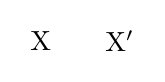
\begin{tikzpicture}
\node [draw=none, inner sep = 1](A) at (0, 0) {X};
\node [draw=none, inner sep = 1] (Y) at (1, 0) {X$^\prime$};
\draw [-latex, draw = white] (A) to (Y);
\end{tikzpicture}
}
\newcommand{\xorx}{
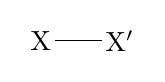
\begin{tikzpicture}
\node [draw=none, inner sep = 1] (A) at (0, 0) {X};
\node [draw=none, inner sep = 1]  (Y) at (1, 0) {X$^{\prime}$};
\draw [draw = black] (A) to (Y);
\end{tikzpicture}
}
\newcommand{\xorxA}{
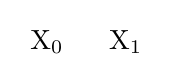
\begin{tikzpicture}
\node [draw=none, inner sep = 1] (A) at (0, 0)  {X$_0$};
\node [draw=none, inner sep = 1]  (Y) at (1, 0)  {X$_1$};
\end{tikzpicture}
}
\newcommand{\xorxorx}{
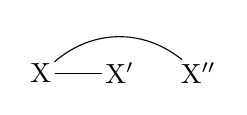
\begin{tikzpicture}
\node [draw=none, inner sep = 1]  (X) at (0, 0) {X};
\node [draw=none, inner sep = 1]  (X1) at (1, 0) {X$^{\prime}$};
\node [draw=none, inner sep = 1] (X2) at (2, 0) {X$^{\prime \prime}$};
\draw [draw = black] (X) to (X1);
\draw [draw = black, bend left = 40] (X) to (X2);
\end{tikzpicture}
}
\newcommand{\xorxchain}{
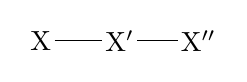
\begin{tikzpicture}
\node [draw=none, inner sep = 1] (X) at (0, 0) {X};
\node [draw=none, inner sep = 1] (X1) at (1, 0) {X$^{\prime}$};
\node [draw=none, inner sep = 1] (X2) at (2, 0) {X$^{\prime \prime}$};
\draw [draw = black] (X) to (X1);
\draw [draw = black] (X1) to (X2);
\end{tikzpicture}
}
\newcommand{\xtox}{

\begin{tikzpicture}
\node [draw=none, inner sep = 1]  (A) at (0, 0)  {X$_\text{parent}$};
\node [draw=none, inner sep = 1]  (Y) at (3, 0)  {X$_\text{child}$};
\draw [-latex, draw = black] (A) to (Y);
\end{tikzpicture}
}
\newcommand{\xtoxA}{
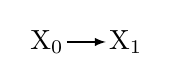
\begin{tikzpicture}
\node [draw=none, inner sep = 1] (A) at (0, 0)  {X$_0$};
\node [draw=none, inner sep = 1]  (Y) at (1, 0)  {X$_1$};
\draw [-latex, draw = black] (A) to (Y);
\end{tikzpicture}
}
\newcommand{\child}{
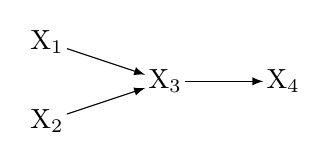
\begin{tikzpicture}
\node [draw=none, inner sep = 1]  (A) at (0, .5) {X$_1$};
\node [draw=none, inner sep = 1]  (L) at (1.5, 0) {X$_3$};
\node [draw=none, inner sep = 1]  (L1) at (3, 0) {X$_4$};
\node [draw=none, inner sep = 1]  (Y) at (0, -.5) {X$_2$};
\draw [-latex, draw = black] (A) to (L);
\draw [-latex, draw = black] (Y) to (L);
\draw [-latex, draw = black] (L) to (L1);
\end{tikzpicture}
}
\newcommand{\fork}{
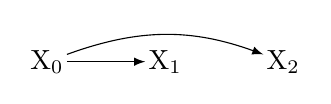
\begin{tikzpicture}
\node [draw=none, inner sep = 1]  (L) at (0, 0) {X$_0$};
\node [draw=none, inner sep = 1]  (A) at (1.5, 0) {X$_1$};
\node [draw=none, inner sep = 1]  (Y) at (3, 0) {X$_2$};
\draw [-latex, draw = black] (L) to (A);
\draw [-latex, draw = white, dotted] (A) to (Y);
\draw [-latex, bend left=20, draw=black] (L) to (Y);
\end{tikzpicture}
}
\newcommand{\chain}{
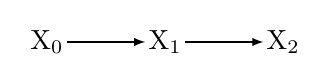
\begin{tikzpicture}
\node [draw=none, inner sep = 1]  (A) at (0, 0) {X$_0$};
\node [draw=none, inner sep = 1] (M) at (1.5, 0) {X$_1$};
\node [draw=none, inner sep = 1]  (Y) at (3, 0) {X$_2$};
\draw [-latex, draw = black] (A) to (M);
\draw [-latex, draw = black] (M) to (Y);
\end{tikzpicture}
}
\newcommand{\immorality}{
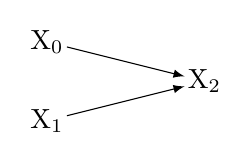
\begin{tikzpicture}
%\node [rectangle, inner sep = 1]  (U) at (0, 0) {};
\node [draw=none, inner sep = 1]  (A) at (1, .5) {X$_0$};
\node [draw=none, inner sep = 1]  (Y) at (1, -.5) {X$_1$};
\node [draw=none, inner sep = 1] (L) at (3, 0) {X$_2$};
\draw [-latex, draw = black] (A) to (L);
\draw [-latex, draw = black] (Y) to (L);
\end{tikzpicture}
}
\newcommand{\network}{
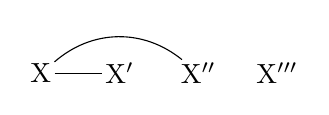
\begin{tikzpicture}
\node [draw=none, inner sep = 1] (X1) at (0, 0) {X};
\node [draw=none, inner sep = 1](X2) at (1, 0) {X$^\prime$};
\node [draw=none, inner sep = 1] (X3) at (2, 0) {X$^{\prime\prime}$};
\node [draw=none, inner sep = 1] (X4) at (3, 0) {X$^{\prime\prime\prime}$};
\draw [draw = black] (X1) to (X2);
\draw [bend left=40, draw=black] (X1) to (X3);
\end{tikzpicture}
}
\newcommand{\aandy}{
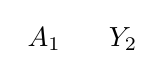
\begin{tikzpicture}
\node [draw=none, inner sep = 0]  (A) at (0, 0) {$A_1$};
\node [draw=none, inner sep = 0]  (Y) at (1, 0) {$Y_2$};
%\node [draw=none, align=center, font=\tiny] at (1.5,.4) {A and Y are not causally associated};
\draw [-latex, draw = white] (A) to (Y);
\end{tikzpicture}
}
\newcommand{\abarandy}{
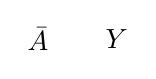
\begin{tikzpicture}
\node [draw=none, inner sep = 0]  (A) at (0, 0) {$\bar{A}$};
\node [draw=none, inner sep = 0]  (Y) at (1, 0) {$Y$};
%\node [draw=none, align=center, font=\tiny] at (1.5,.4) {A and Y are not causally associated};
\draw [-latex, draw = white] (A) to (Y);
\end{tikzpicture}
}
\newcommand{\atoy}{
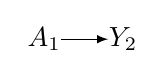
\begin{tikzpicture}
\node [draw=none, inner sep = 0] (A) at (0, 0) {$A_1$};
\node [draw=none, inner sep = 0] (Y) at (1, 0) {$Y_2$};
\draw [-latex, draw = black] (A) to (Y);
%\node [draw=none, align=center, font=\tiny] at (1.25,.4) {A and Y are causally associated};
\end{tikzpicture}
}
\newcommand{\atoyLONG}{
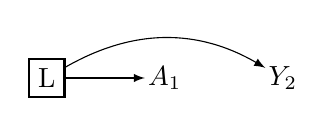
\begin{tikzpicture}
\node [rectangle,  draw=black, thick] (L) at (0, 0) {L};
\node [draw=none, inner sep = 1] (A) at (1.5, 0) {$A_1$};
\node [draw=none, inner sep = 1] (Y) at (3, 0) {$Y_2$};
\draw [-latex, draw = black] (L) to (A);
\draw [-latex, draw = black, bend left = 30] (L) to (Y);
%\node [draw=none, align=center, font=\tiny] at (1.25,.4) {A and Y are causally associated};
\end{tikzpicture}
}
\newcommand{\abartoy}{
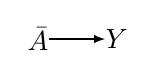
\begin{tikzpicture}
\node [draw=none, inner sep = 0] (A) at (0, 0) {$\bar{A}$};
\node [draw=none, inner sep = 0] (Y) at (1, 0) {$Y$};
\draw [-latex, draw = black] (A) to (Y);
%\node [draw=none, align=center, font=\tiny] at (1.25,.4) {A and Y are causally associated};
\end{tikzpicture}
}
\newcommand{\immoralityChild}{
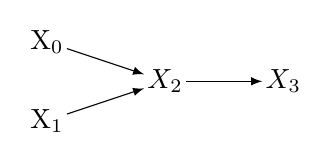
\begin{tikzpicture}
\node [draw = none, inner sep = 1] (A) at (0, .5) {X$_0$};
\node [draw = none, inner sep = 1] (Y) at (0, -.5) {X$_1$};
\node [draw = none, inner sep = 1] (L) at (1.5, 0) {$X_2$};
\node [draw = none, inner sep = 1] (L1) at (3, 0) {$X_3$};
\draw [-latex, draw = black] (A) to (L);
\draw [-latex, draw = black] (Y) to (L);
\draw [-latex, draw = black] (L) to (L1);
\end{tikzpicture}
}
\newcommand{\atoybiased}{
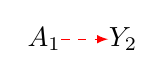
\begin{tikzpicture}
\node [draw=none, inner sep = 0]  (A) at (0, 0) {$A_1$};
\node [draw=none, inner sep = 0]  (Y) at (1.0, 0) {$Y_2$};
%\node [draw=none, align=center, font=\tiny] at (1.5,.4) {Bias in causal association of A and Y};
\draw [-latex, draw = red, dashed] (A) to (Y);
\end{tikzpicture}
}
\newcommand{\abartoybiased}{
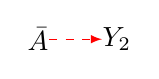
\begin{tikzpicture}
\node [draw=none, inner sep = 0]  (A) at (0, 0) {$\bar{A}$};
\node [draw=none, inner sep = 0]  (Y) at (1.0, 0) {$Y_2$};
%\node [draw=none, align=center, font=\tiny] at (1.5,.4) {Bias in causal association of A and Y};
\draw [-latex, draw = red, dashed] (A) to (Y);
\end{tikzpicture}
}
\newcommand{\atoybiasedA}{
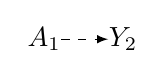
\begin{tikzpicture}
\node [draw=none, inner sep = 0]  (A) at (0, 0) {$A_1$};
\node [draw=none, inner sep = 0]  (Y) at (1.0, 0) {$Y_2$};
%\node [draw=none, align=center, font=\tiny] at (1.5,.4) {Estimates Direct Effect of A on Y};
\draw [-latex, draw = black, dashed] (A) to (Y);
\end{tikzpicture}
}
\newcommand{\atoybiasedB}{
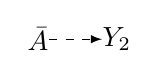
\begin{tikzpicture}
\node [draw=none, inner sep = 0]  (A) at (0, 0) {$\bar{A}$};
\node [draw=none, inner sep = 0]  (Y) at (1.0, 0) {$Y_2$};
%\node [draw=none, align=center, font=\tiny] at (1.5,.4) {Estimates Direct Effect of A on Y};
\draw [-latex, draw = black, dashed] (A) to (Y);
\end{tikzpicture}
}
\newcommand{\ytoa}{
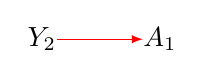
\begin{tikzpicture}
%\node [draw=none, align=center, font=\small] at (0,1) {\bf Timing};
\node [draw=none, inner sep = 0] (Y) at (0, 0) {$Y_2$};
\node [draw=none, inner sep = 0] (A) at (1.5, 0) {$A_1$};
\draw [-latex, red] (Y) to (A);
\end{tikzpicture}
}
\newcommand{\atwotoyone}{
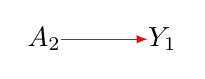
\begin{tikzpicture}
%\node [draw=none, align=center, font=\small] at (0,1) {\bf Timing};
\node [draw=none, inner sep = 0]  (A) at (0, 0) {$A_2$};
\node [draw=none, inner sep = 0]  (Y) at (1.5, 0) {$Y_1$};
\draw [-latex, draw = red] (A) to (Y);
\end{tikzpicture}
}
\newcommand{\commoncause}{
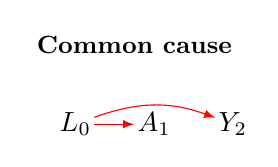
\begin{tikzpicture}
\node [draw=none, align=center, font=\small] at (.75,1) {\bf Common cause};
\node [draw = none, inner sep = 1] (L) at (0, 0) {$L_0$};
\node [draw = none, inner sep = 1] (A) at (1, 0) {$A_1$};
\node [draw = none, inner sep = 1] (Y) at (2, 0) {$Y_2$};
\draw [-latex, draw = red] (L) to (A);
\draw [-latex, draw = white, dotted] (A) to (Y);
\draw [-latex, bend left=20, draw=red] (L) to (Y);
\end{tikzpicture}
}
\newcommand{\commoncauseA}{
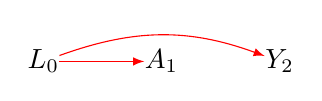
\begin{tikzpicture}
%\node [draw=none, align=center, font=\small] at (.75,1) {\bf Common cause};
\node [draw=none, inner sep = 0] (L) at (0, 0) {$L_0$};
\node [draw=none, inner sep = 0] (A) at (1.5, 0) {$A_1$};
\node [draw=none, inner sep = 0] (Y) at (3, 0) {$Y_2$};
\draw [-latex, draw = red] (L) to (A);
\draw [-latex, draw = white, dotted] (A) to (Y);
\draw [-latex, bend left=20, draw=red] (L) to (Y);
\end{tikzpicture}
}
\newcommand{\commoncauseAshort}{
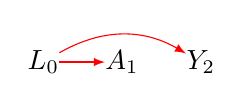
\begin{tikzpicture}
\node [draw=none, inner sep = 0] (L) at (0, 0) {$L_0$};
\node [draw=none, inner sep = 0] (A) at (1, 0) {$A_1$};
\node [draw=none, inner sep = 0] (Y) at (2, 0) {$Y_2$};
\draw [-latex, draw = red] (L) to (A);
\draw [-latex, draw = white, dotted] (A) to (Y);
\draw [-latex, bend left=30, draw=red] (L) to (Y);
\end{tikzpicture}
}
\newcommand{\commoncauseAA}{
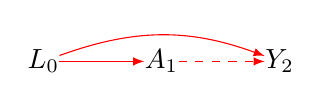
\begin{tikzpicture}
%\node [draw=none, align=center, font=\small] at (.75,1) {\bf Common cause};
\node [draw=none, inner sep = 0] (L) at (0, 0) {$L_0$};
\node [draw=none, inner sep = 0] (A) at (1.5, 0) {$A_1$};
\node [draw=none, inner sep = 0] (Y) at (3, 0) {$Y_2$};
\draw [-latex, draw = red] (L) to (A);
\draw [-latex, draw = red, dashed] (A) to (Y);
\draw [-latex, bend left=20, draw=red] (L) to (Y);
\end{tikzpicture}
}
\newcommand{\commoncauseALATENTshort}{
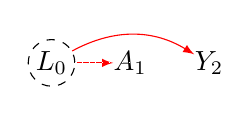
\begin{tikzpicture}
%\node [draw=none, align=center, font=\small] at (1.25,1) {\bf Condition on pre-exposure L};
\node [circle, draw=black, dashed, inner sep = 1] (U) at (0, 0) {$L_0$};
\node [draw=none, inner sep = 0]  (A) at (1, 0) {$A_1$};
\node [draw=none, inner sep = 0]  (Y) at (2, 0) {$Y_2$};
\draw [-latex, draw = red] (U) to (A);
\draw [-latex, draw = white, dotted] (U) to (Y);
\draw [-latex, bend left=30, draw=red] (U) to (Y);
\end{tikzpicture}
}
\newcommand{\mediator}{
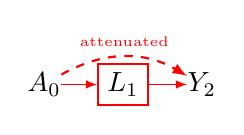
\begin{tikzpicture}
%\node [draw=none, align=center, font=\small] at (.25,1) {\bf Mediator bias};
\node [draw=none, inner sep = 0]  (A) at (0, 0) {$A_0$};
\node [rectangle, draw=red, thick] (L) at (1, 0) {$L_1$};
\node [draw=none, inner sep = 0] (Y) at (2, 0) {$Y_2$};
\draw [-latex, draw = red] (A) to (L);
\draw [-latex, draw = red] (L) to (Y);
\draw [-latex,  bend left=30, draw=red,dashed, thick] (A) to node[pos=0.5, above,draw=none, text = red] {\tiny attenuated} (Y);
\end{tikzpicture}
}
\newcommand{\mediatorA}{
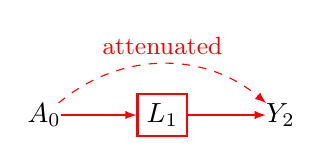
\begin{tikzpicture}
%\node [draw=none, align=center, font=\small] at (.25,1) {\bf Mediator bias};
\node [draw=none, inner sep = 0](A) at (0, 0) {$A_0$};
\node [rectangle, draw=red, thick] (L) at (1.5, 0) {$L_1$};
\node [draw=none, inner sep = 0] (Y) at (3, 0) {$Y_2$};
\draw [-latex, draw = red] (A) to (L);
\draw [-latex, draw = red] (L) to (Y);
\draw [-latex,  bend left=40, draw=red,dashed] (A) to node[pos=0.5, above,draw=none, text = red] {\small attenuated} (Y);
\end{tikzpicture}
}
\newcommand{\collider}{
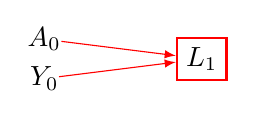
\begin{tikzpicture}
%\node [draw=none, align=center, font=\small] at (0,.75) {\bf Collider};
\node [draw=none, inner sep = 0]  (A) at (0, .25) {$A_0$};
\node [rectangle,  draw=red, thick] (L) at (2, 0) {$L_1$};
\node [draw=none, inner sep = 0]  (Y) at (0, -.25) {$Y_0$};
\draw [-latex, draw = red] (A) to (L);
\draw [-latex, draw = red] (Y) to (L);
\end{tikzpicture}
}
\newcommand{\colliderA}{
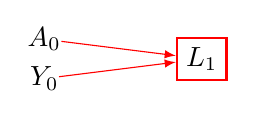
\begin{tikzpicture}
%node [draw=none, align=center, font=\small] at (0,.75) {\bf Collider};
\node [draw=none, inner sep = 0]  (A) at (0, .25) {$A_0$};
\node [rectangle,  draw=red, thick] (L) at (2, 0) {$L_1$};
\node [draw=none, inner sep = 0] (Y) at (0, -.25) {$Y_0$};
\draw [-latex, draw = red] (A) to (L);
\draw [-latex, draw = red] (Y) to (L);
\end{tikzpicture}
}
\newcommand{\colliderALONG}{
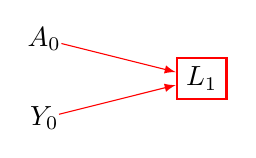
\begin{tikzpicture}
%node [draw=none, align=center, font=\small] at (0,.75) {\bf Collider};
\node [draw=none, inner sep = 0]  (A) at (0, .5) {$A_0$};
\node [rectangle,  draw=red, thick] (L) at (2, 0) {$L_1$};
\node [draw=none, inner sep = 0] (Y) at (0, -.5) {$Y_0$};
\draw [-latex, draw = red] (A) to (L);
\draw [-latex, draw = red] (Y) to (L);
\end{tikzpicture}
}
\newcommand{\descendantB}{
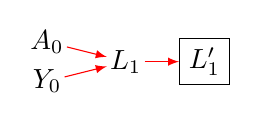
\begin{tikzpicture}
%\node [draw=none, align=center, font=\small] at (1.5,.75) {\bf Descendant of collider};
\node [draw = none, inner sep = 1] (A) at (0, .25) {$A_0$};
\node [draw = none, inner sep = 1] (L) at (1, 0) {$L_1$};
\node [rectangle, draw=black] (L1) at (2, 0) {$L'_1$};
\node [draw = none, inner sep = 1] (Y) at (0, -.25) {$Y_0$};
\draw [-latex, draw = red] (A) -- (L);
\draw [-latex, draw = red] (Y) -- (L);
\draw [-latex, draw = red] (L) -- (L1);
\end{tikzpicture}
}
\newcommand{\descendantBB}{
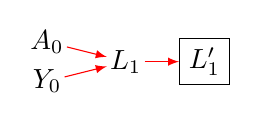
\begin{tikzpicture}
%\node [draw=none, align=center, font=\small] at (1.5,.75) {\bf Descendant of collider};
\node [draw = none, inner sep = 1] (A) at (0, .25) {$A_0$};
\node [draw = none, inner sep = 1] (L) at (1, 0) {$L_1$};
\node [rectangle, draw=black] (L1) at (2, 0) {$L'_1$};
\node [draw = none, inner sep = 1] (Y) at (0, -.25) {$Y_0$};
\draw [-latex, draw = red] (A) -- (L);
\draw [-latex, draw = red] (Y) -- (L);
\draw [-latex, draw = red] (L) -- (L1);
\end{tikzpicture}
}

\newcommand{\descendantBBLONG}{
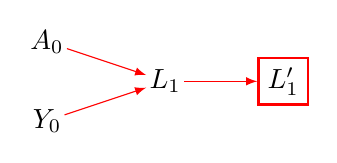
\begin{tikzpicture}
%\node [draw=none, align=center, font=\small] at (1.5,.75) {\bf Descendant of collider};
\node [draw = none, inner sep = 1] (A) at (0, .5) {$A_0$};
\node [draw = none, inner sep = 1] (Y) at (0, -.5) {$Y_0$};
\node [draw = none, inner sep = 1] (L) at (1.5, 0) {$L_1$};
\node [rectangle, draw=red, thick] (L1) at (3, 0) {$L'_1$};
\draw [-latex, draw = red] (A) -- (L);
\draw [-latex, draw = red] (Y) -- (L);
\draw [-latex, draw = red] (L) -- (L1);
\end{tikzpicture}
}
\newcommand{\mediatorcollider}{
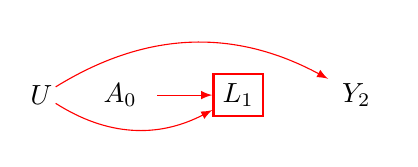
\begin{tikzpicture}
%\node [draw=none, align=center, font=\small] at (2,1) {\bf Condition on child of collider};
\node [draw = none, inner sep = 1] (U) at (0, 0) {$U$};
\node [ellipse, draw=white] (A) at (1, 0) {$A_{0}$};
\node [rectangle, draw=red, thick](L) at (2.5, 0) {$L_{1}$};
\node [ellipse, draw=white] (Y) at (4, 0) {$Y_{2}$};
\draw [-latex, bend right=30, draw = red] (U) to (L);
\draw [-latex, bend left = 30, draw=red] (U) to (Y);
\draw [-latex,draw=red] (A) to (L);
\end{tikzpicture}
}
\newcommand{\downstreamconfounder}{
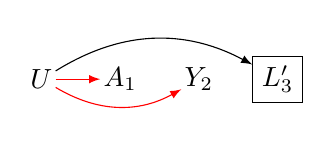
\begin{tikzpicture}
%\node [draw=none, align=center, font=\small] at (2.5,1) {\bf Condition on child of unmeasured confounder};
\node [draw=none, inner sep = 1] (U) at (0, 0) {$U$};
\node [draw=none, inner sep = 1] (A) at (1, 0) {$A_{1}$};
\node [draw=none, inner sep = 1] (Y) at (2, 0) {$Y_{2}$};
\node [rectangle, draw=black] (L) at (3, 0) {$L^{\prime}_{3}$};
\draw [-latex, bend right=30, draw =red] (U) to (Y);
\draw [-latex, bend left = 30, draw=black] (U) to (L);
\draw [-latex, draw =red] (U) to (A);
\end{tikzpicture}
}
\newcommand{\downstream}{
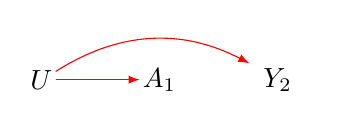
\begin{tikzpicture}
%\node [draw=none, align=center, font=\small] at (1.25,1) {\bf Unmeasured confounding};
\node [draw=none, inner sep = 1] (U) at (0, 0) {$U$};
\node [draw = none, inner sep = 1](A) at (1.5, 0) {$A_{1}$};
\node [ellipse, draw=white] (Y) at (3, 0) {$Y_{2}$};
\draw [-latex, bend left=30, draw =red] (U) to (Y);
\draw [-latex, draw =red] (U) to (A);
\end{tikzpicture}
}
\newcommand{\mediatorm}{
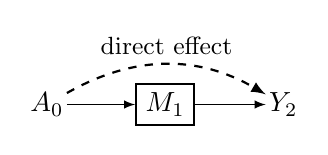
\begin{tikzpicture}
\node [draw=none,inner sep = 1] (A) at (0, 0) {$A_0$};
\node [rectangle, draw=black, thick] (M) at (1.5, 0) {$M_1$};
\node [draw=none,inner sep = 1] (Y) at (3, 0) {$Y_2$};
\draw [-latex, draw = black] (A) to (M);
\draw [-latex, draw = black] (M) to (Y);
\draw [-latex,  bend left=30, draw=black, dashed, thick] (A) to node[pos=0.5, above, draw=none, text = black] {\small direct effect} (Y);
\end{tikzpicture}
}
\newcommand{\mediatormSHORT}{
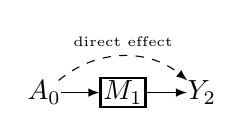
\begin{tikzpicture}
\node [draw=none, inner sep = 0]  (A) at (0, 0) {$A_0$};
\node [rectangle, draw=black, thick,inner sep = 1] (M) at (1, 0) {$M_1$};
\node [draw=none, inner sep = 0]  (Y) at (2, 0) {$Y_2$};
\draw [-latex, draw = black] (A) to (M);
\draw [-latex, draw = black] (M) to (Y);
\draw [-latex,  bend left=40, draw=black, dashed] (A) to node[pos=0.5, above, draw=none, text = black] {\tiny direct effect} (Y);
\end{tikzpicture}
}
\newcommand{\mbias}{
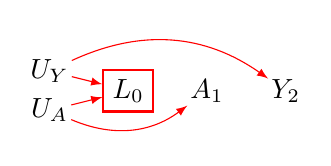
\begin{tikzpicture}
%\node [draw=none, align=center, font=\small] at (-.25,1) {\bf M-bias};
\node [draw=none, align=center, inner sep = 1](UA) at (0, -.25) {$U_A$};
\node [draw=none, align=center, inner sep = 1] (UY) at (0, .25) {$U_Y$};
\node [rectangle,  draw=red, thick] (L) at (1, 0) {$L_0$};
\node [draw=none, align=center, inner sep = 1](A) at (2, 0) {$A_1$};
\node [draw=none, align=center, inner sep = 1] (Y) at (3, 0) {$Y_2$};
\draw [-latex, draw = red] (UA) to (L);
\draw [-latex, draw = red] (UY) to (L);
\draw [-latex, draw = red, bend right = 30] (UA) to (A);
\draw [-latex, draw = red, bend left = 30] (UY) to (Y);
\end{tikzpicture}
}
\newcommand{\mbiasdoomed}{
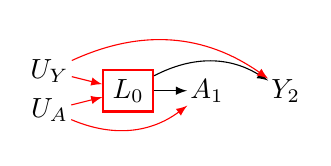
\begin{tikzpicture}
%\node [draw=none, align=center, font=\small] at (1.25,1) {\bf M-bias, L is confounder};
\node [draw=none, align=center, inner sep = 1](UA) at (0, -.25) {$U_A$};
\node [draw=none, align=center, inner sep = 1] (UY) at (0, .25) {$U_Y$};
\node [rectangle,  draw=red, thick] (L) at (1, 0) {$L_0$};
\node [draw=none, align=center, inner sep = 1] (A) at (2, 0) {$A_1$};
\node [draw=none, align=center, inner sep = 1](Y) at (3, 0) {$Y_2$};
\draw [-latex, draw = black] (L) to (A);
\draw [-latex, draw = black, bend left = 30] (L) to (Y);
\draw [-latex, draw = red] (UA) to (L);
\draw [-latex, draw = red] (UY) to (L);
\draw [-latex, draw = red, bend right = 30] (UA) to (A);
\draw [-latex, draw = red, bend left = 30] (UY) to (Y);
\end{tikzpicture}
}
% solutions 
\newcommand{\aandysolution}{
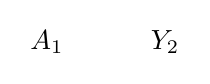
\begin{tikzpicture}
%\node [draw=none, align=left, font=\small] at (1.25,1) {\bf Ensure relative timing of A and Y};
\node [draw = none, inner sep = 1] (A) at (0, 0) {$A_1$};
\node [draw = none, inner sep = 1] (Y) at (1.5, 0) {$Y_2$};
\draw [-latex, draw = white] (A) to (Y);
\end{tikzpicture}
}
\newcommand{\aandygenderalsolution}{
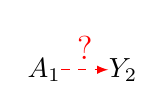
\begin{tikzpicture}
\node [draw=none, inner sep = 0] (A) at (0, 0) {$A_1$};
\node [draw=none, inner sep = 0]  (Y) at (1, 0) {$Y_2$};
\draw [-latex, draw = red, dashed] (A) to  node[pos=0.5, above, draw=none, text= red] {\large ?}(Y);
\end{tikzpicture}
}
\newcommand{\commoncausesolved}{
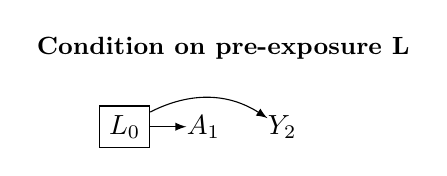
\begin{tikzpicture}
\node [draw=none, align=center, font=\small] at (1.25,1) {\bf Condition on pre-exposure L};
\node [rectangle, draw=black] (L) at (0, 0) {$L_0$};
\node [draw=none, inner sep = 0] (A) at (1, 0) {$A_1$};
\node [draw=none, inner sep = 0]  (Y) at (2, 0) {$Y_2$};
\draw [-latex, draw = black] (L) to (A);
\draw [-latex, draw = white, dotted] (A) to (Y);
\draw [-latex, bend left=30, draw=black] (L) to (Y);
\end{tikzpicture}
}
\newcommand{\commoncausesolvedA}{
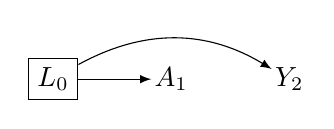
\begin{tikzpicture}
%\node [draw=none, align=center, font=\small] at (1.25,1) {\bf Condition on pre-exposure L};
\node [rectangle, draw=black] (L) at (0, 0) {$L_0$};
\node [draw = none, inner sep = 1] (A) at (1.5, 0) {$A_1$};
\node [draw = none, inner sep = 1] (Y) at (3, 0) {$Y_2$};
\draw [-latex, draw = black] (L) to (A);
\draw [-latex, draw = white, dotted] (A) to (Y);
\draw [-latex, bend left=30, draw=black] (L) to (Y);
\end{tikzpicture}
}
\newcommand{\commoncausesolvedAshort}{
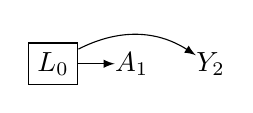
\begin{tikzpicture}
%\node [draw=none, align=center, font=\small] at (1.25,1) {\bf Condition on pre-exposure L};
\node [rectangle, draw=black] (L) at (0, 0) {$L_0$};
\node [draw=none, inner sep = 0]  (A) at (1, 0) {$A_1$};
\node [draw=none, inner sep = 0]  (Y) at (2, 0) {$Y_2$};
\draw [-latex, draw = black] (L) to (A);
\draw [-latex, draw = white, dotted] (A) to (Y);
\draw [-latex, bend left=30, draw=black] (L) to (Y);
\end{tikzpicture}
}
\newcommand{\mbiassolved}{
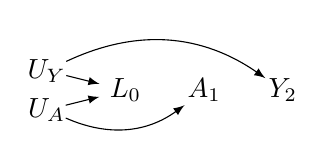
\begin{tikzpicture}
%\node [draw=none, align=center, font=\small] at (1,1) {\bf Do not condition on L};
\node [draw=none, inner sep = 0]  (UA) at (0, -.25) {$U_A$};
\node [draw=none, inner sep = 0]  (UY) at (0, .25) {$U_Y$};
\node [rectangle,  draw=white, thick] (L) at (1, 0) {$L_0$};
\node [draw = none, inner sep = 1] (A) at (2, 0) {$A_1$};
\node [draw = none, inner sep = 1] (Y) at (3, 0) {$Y_2$};
\draw [-latex, draw = black] (UA) to (L);
\draw [-latex, draw = black] (UY) to (L);
\draw [-latex, draw = black, bend right = 30] (UA) to (A);
\draw [-latex, draw = black, bend left = 30] (UY) to (Y);
\end{tikzpicture}
}
\newcommand{\commoncausesolvedchild}{
\begin{tikzpicture}
%\node [draw=none, align=center, font=\small] at (.25,1) {\bf Condition on pre-exposure L$^\prime$};
\node [draw=none, align=center, inner sep = 1](U) at (-1, 0) {$U$};
\node [rectangle, draw=black] (L1) at (0, 0) {$L^{\prime}_0$};
\node [draw=none, align=center, inner sep = 1] (A) at (1, 0) {$A_1$};
\node [draw=none, align=center, inner sep = 1] (Y) at (2, 0) {$Y_2$};                        
\draw [-latex, draw = black] (U) to (L1);
\draw [-latex, draw = black] (L1) to (A);
\draw [-latex, draw = black, bend left = 30] (U) to (Y);
\end{tikzpicture}
}
\newcommand{\mbiasdoomedsolved}{
\begin{tikzpicture}
%\node [draw=none, font=\small] at (1.25, 1) {\bf Condition on measured child of UA OR UY};
\node [draw=none, align=center, inner sep = 1](UA) at (0, -.5) {$U_A$};
\node [draw=none, align=center, inner sep = 1](UY) at (0, .25) {$U_Y$};
\node [rectangle,  draw=black, inner sep = 2] (L) at (1.5, 0) {$L_0$};
\node [rectangle,  draw=red, inner sep = 2] (L1) at (1.5, .5) {$L^{UY}$};
\node [draw=none, align=center, inner sep = 1] (A) at (2.5, 0) {$A_1$};
\node [draw=none, align=center, inner sep = 1] (Y) at (3.5, 0) {$Y_2$};
\draw [-latex, draw = black] (UA) to (L);
\draw [-latex, draw = black] (UY) to (L);
\draw [-latex, draw = black] (L) to (A);
\draw [-latex, draw = black, bend left = 20] (L) to (Y);
\draw [-latex, draw = black, bend right = 10] (UA) to (A);
\draw [-latex, draw = black] (UY) to (L1);
\end{tikzpicture}
}
\newcommand{\effectmodifierA}{
\begin{tikzpicture}
\node [rectangle,  inner sep=4pt,  draw=blue, thick] (Z) at (0,0) {$Z$};
\node [draw = none, inner sep = 1] (A) at (1.5, 0) {$A_1$};
\node [draw = none, inner sep = 1] (Y) at (3, 0) {$Y_2$};
\draw [-latex, draw = blue, bend left = 20] (Z) to (Y);
\draw [-latex, draw = black] (A) to (Y);
\end{tikzpicture}
}
\newcommand{\effectmodifierB}{
\begin{tikzpicture}
\node [circle,  inner sep=4pt,  draw=blue, dashed] (Z) at (0,0) {Z};
\node [draw = none, inner sep = 1] (A) at (1.5, 0) {$A_1$};
\node [draw = none, inner sep = 1] (Y) at (3, 0) {$Y_2$};
\draw [-latex, draw = blue, bend left = 20] (Z) to (Y);
\draw [-latex, draw = black] (A) to (Y);
\end{tikzpicture}
}
\newcommand{\effectmodifierC}{
\begin{tikzpicture}
\node [circle, inner sep=6pt, draw=blue,align=left, thick, dashed] (Z) at (0, 0) {$Z$};
\node [rectangle] (A) at (1.5, 0) {$A_1$};
\node [circle, inner sep=4pt,  thick, dashed, draw = black, text=black] (Y) at (3.5,0) {$Y_2$};
\node [circle, inner sep=2pt, draw=blue, text=black, dashed, thick] (US) at (5.5, 1.5) {$U_{\Delta Z \rightarrowblueB Y'}$};
\node [rectangle, draw=black, thick, red, text=black](YS) at (5.5, 0) {Y$_2^{S=1}$};
\draw [-latex, draw=black] (A) to node[pos=0.5, above, draw=none, text = black] {\tiny target}(Y);
\draw [-latex, draw=red] (Y) to node[pos=0.5, above, draw=none, text = red] {\tiny bias}(YS);
\draw [-latex, draw=black] (US) to (YS);
\draw [-latex,bend left=40, blue] (Z) to (Y);
\end{tikzpicture}
}
%measurement
\newcommand{\measurementerroruncorrelated}{
\begin{tikzpicture}
\node [circle, inner sep=2pt, draw=black, dashed, inner sep = 1] (A) at (0, 0) {$A_1$};
\node [rectangle, draw=red, inner sep = 2]  (A1) at (0, 1.5) {$A'$};
\node [circle, inner sep=2pt, draw=black, dashed, inner sep = 1] (Y) at (2, 0) {$Y_2$};
\node [rectangle, draw=red, inner sep = 2] (Y1) at (2, 1.5) {$Y'$};
\draw [-latex, draw = red, dashed] (A) to node[pos=0.5, sloped, above, draw=none, text= black] {\tiny error} (A1);
\draw [-latex, draw = red, dashed] (Y) to node[pos=0.5, sloped, above, draw=none, text= black] {\tiny error} (Y1);
\draw [-latex, draw = black] (A) to node[pos=0.5, above, draw=none, text= black] {\tiny truth} (Y);
\draw [-latex, draw = red, dashed, thick] (A1) to node[pos=0.5, sloped, above, draw=none, text=black] {\tiny distorted} (Y1);
\end{tikzpicture}
}
\newcommand{\measurementUNCOR}{
\begin{tikzpicture}
\node [circle, inner sep=2pt, draw=white] (UA) at (0, 0) {$U_A$};
\node [circle, inner sep=2pt, draw=black, dashed] (A) at (2, 0) {$A_1$};
\node [rectangle, draw=black,thick] (A1) at (4, 0) {$A'_1$};
\node [draw = none, inner sep = 1] (UY) at (6, 0) {$U_Y$};
\node [circle,  inner sep=2pt, draw=black, dashed] (Y) at (8, 0) {$Y_2$};
\node [rectangle, draw=black, thick] (Y1) at (10, 0) {$Y'_2$};
\draw [-latex, draw = black, bend left = 40] (UA) to (A1);
\draw [-latex, draw = black] (A) to (A1);
\draw [-latex, draw = black] (Y) to (Y1);
\draw [-latex, draw = black, bend left = 40] (UY) to (Y1);
\end{tikzpicture}
}
\newcommand{\measurementUCORB}{
\begin{tikzpicture}
\node [circle, draw=blue, dashed, thick] (UA) at (0, 0) {$U_{A}$};
\node [circle, draw=black, dashed] (A) at (2, 0) {$A_1$};
\node [rectangle, draw=red, thick] (A1) at (4, 0) {$A'_1$};
\node [circle, draw=blue, dashed, thick] (UY) at (6, 0) {$U_{Y}$};
\node [circle, draw=black, dashed] (Y) at (8, 0) {$Y_2$};
\node [rectangle, draw=red, thick] (Y1) at (10, 0) {$Y'_2$};
\draw [-latex, draw = blue, bend left = 40] (UA) to (A1);
\draw [-latex, draw = black] (A) to (A1);
\draw [-latex, draw = black] (Y) to (Y1);
\draw [-latex, draw = blue, bend left = 40] (UY) to (Y1);
\draw [-latex, bend right = 40, draw = black] (A) to node[pos=0.5, below, draw=none] {\tiny target}(Y);
\draw [-latex, bend left = 40, draw = red,  dashed, thick] (A1) to node[pos=0.5, above, draw=none, text= red] {\tiny biased}(Y1);
\end{tikzpicture}
}
\newcommand{\measurementCOR}{
\begin{tikzpicture}
\node [draw = none, inner sep = 1] (U) at (0, 0) {$U_{AY}$};
\node [circle, draw=black, dashed] (A) at (1.25, 0) {$A_1$};
\node [rectangle, draw=red, thick] (A1) at (3, 0) {$A'_1$};
\node [circle, draw=black, dashed] (Y) at (4.5, 0) {$Y_2$};
\node [rectangle, draw=red, thick] (Y1) at (6, 0) {$Y'_2$};
\draw [-latex, draw = red, bend left = 30] (U) to (A1);
\draw [-latex, draw = black] (A) to (A1);
\draw [-latex, draw = red, bend left = 30] (U) to (Y1);
\draw [-latex, draw = black] (Y) to (Y1);
\end{tikzpicture}
}
\newcommand{\measurementDIR}{
\begin{tikzpicture}
\node [draw = none, inner sep = 1] (UA) at (0, 0) {$U_A$};
\node [circle, draw=black, dashed] (A) at (1.5, 0) {$A_1$};
\node [rectangle,draw=red, thick] (A1) at (3, 0) {$A'_1$};
\node [draw = none, inner sep = 1] (UY) at (4.5, 0) {$U_Y$};
\node [circle, draw=black, dashed] (Y) at (6, 0) {$Y_2$};
\node [rectangle, draw=red, thick] (Y1) at (7.5, 0) {$Y'_2$};
\draw [-latex, draw = black,  bend right = 40] (UA) to (A1);
\draw [-latex, draw = red] (A) to (A1);
\draw [-latex, draw = red, bend left = 40] (A) to (UY);
\draw [-latex, draw =black] (Y) to (Y1);
\draw [-latex, draw = red, bend right = 40] (UY) to (Y1);
\end{tikzpicture}
}
\newcommand{\measurementCORDIR}{
\begin{tikzpicture}
\node [draw = none, inner sep = 1] (UAY) at (0, 0) {$U_{AY}$};
\node [draw = none, inner sep = 1] (UA) at (1.5, 0) {$U_A$};
\node [circle, draw=black, dashed] (A) at (3, 0) {$A_1$};
\node [rectangle, draw=red, thick] (A1) at (4.5, 0) {$A'_1$};
\node [draw = none, inner sep = 1] (UY) at (6, 0) {$U_Y$};
\node [circle, draw=black, dashed] (Y) at (7, 0) {$Y_2$};
\node [rectangle, draw=red, thick] (Y1) at (9, 0) {$Y'_2$};
\draw [-latex, draw = red] (UAY) to (UA);
\draw [-latex, draw = red, bend right = 40] (UA) to (A1);
\draw [-latex, draw = red] (A) to (A1);
\draw [-latex, draw = red,bend right = 40] (UY) to (Y1);
\draw [-latex, draw = black] (Y) to (Y1);
\draw [-latex, draw = red, bend left = 40] (A) to (UY);
\draw [-latex, draw = red, bend left = 40] (UAY) to (UY);
\end{tikzpicture}
}
\newcommand{\measurementY}{
\begin{tikzpicture}
\node [circle, draw=black, dashed] (A) at (0, 0) {$A_1$};
\node [circle, draw=black, dashed] (Y) at (1.5, 0) {$Y_2$};
\node [draw = none, inner sep = 1] (UA) at (3, 0) {$U_A$};
\node [rectangle, draw=red, thick] (A1) at (4.5, 0) {$A'$};
\node [draw = none, inner sep = 1] (UY) at (6, 0) {$U_Y$};
\node [rectangle,  draw=red, thick] (Y1) at (7.5, 0) {$Y'$};
\draw [-latex, draw = red] (Y) to (UA);
\draw [-latex, draw = red] (UA) to (A1);
\draw [-latex, draw = black, bend right = 30] (A) to (A1);
\draw [-latex, draw = black] (UY) to (Y1);
\draw [-latex, draw = red, bend left = 30] (Y) to (Y1);
\end{tikzpicture}
}
\newcommand{\measurementUNCORshort}{
\begin{tikzpicture}
\node [draw = none, inner sep = 1] (UA) at (0, 0) {$U_A$};
\node [circle, inner sep=1pt, draw=black, dashed] (A) at (1.5, 0) {$A_1$};
\node [rectangle, draw=black, thick] (A1) at (3, 0) {$A'_1$};
\node [draw = none, inner sep = 1] (UY) at (5, 0) {$U_Y$};
\node [circle,  inner sep=1pt, draw=black, dashed] (Y) at (6.5, 0) {$Y_2$};
\node [rectangle, draw=black, thick] (Y1) at (8, 0) {$Y'_2$};
\draw [-latex, draw = black, bend left = 40] (UA) to (A1);
\draw [-latex, draw = black] (A) to (A1);
\draw [-latex, draw = black] (Y) to (Y1);
\draw [-latex, draw = black, bend left = 40] (UY) to (Y1);
\end{tikzpicture}
}
\newcommand{\measurementUCORBshort}{
\begin{tikzpicture}
\node [circle, draw = blue, inner sep = 4, dashed] (UA) at (0, 0) {$U_A$};
\node [circle, inner sep=2pt, draw=black, dashed] (A) at (1.5, 0) {$A_1$};
\node [rectangle, draw=black] (A1) at (3, 0) {$A'_1$};
\node [circle, draw = blue, inner sep = 4, dashed]  (UY) at (5, 0) {$U_Y$};
\node [circle,  inner sep=2pt, draw=black, dashed] (Y) at (7, 0) {$Y_2$};
\node [rectangle, draw=black] (Y1) at (9, 0) {$Y'_2$};
\draw [-latex, draw = blue, bend left = 30] (UA) to (A1);
\draw [-latex, draw = blue] (A) to (A1);
\draw [-latex, draw = blue] (Y) to (Y1);
\draw [-latex, draw = blue, bend left = 30] (UY) to (Y1);
%\draw [-latex, draw = blue, bend right = 30, thick] (UA) to (Y1);
\draw [-latex, bend right = 30, draw = black] (A) to node[pos=0.5, above, draw=none] {\tiny target}(Y);
\draw [-latex, bend left = 30, draw = red,  dashed] (A1) to node[pos=0.5, above, draw=none, text= red] {\tiny biased for target}(Y1);
\end{tikzpicture}
}
\newcommand{\measurementCORshort}{
\begin{tikzpicture}
\node [draw = none, inner sep = 1] (U) at (0, 0) {$U_{AY}$};
\node [circle, draw=black, dashed] (A) at (2, 0) {$A_1$};
\node [rectangle, draw=red] (A1) at (4, 0) {$A'_1$};
\node [circle, draw=black, dashed] (Y) at (6, 0) {$Y_2$};
\node [rectangle, draw=red] (Y1) at (9, 0) {$Y'_2$};
\draw [-latex, draw = red, bend left = 30] (U) to (A1);
\draw [-latex, draw = black] (A) to (A1);
\draw [-latex, draw = red, bend left = 30] (U) to (Y1);
\draw [-latex, draw = black] (Y) to (Y1);
\end{tikzpicture}
}
\newcommand{\measurementDIRshort}{
\begin{tikzpicture}
\node [draw = none, inner sep = 1] (UA) at (0, 0) {$U_A$};
\node [circle, draw=black, dashed] (A) at (2, 0) {$A_1$};
\node [rectangle,draw=red] (A1) at (4, 0) {$A'_1$};
\node [draw = none, inner sep = 1] (UY) at (6, 0) {$U_Y$};
\node [circle, draw=black, dashed] (Y) at (7.5, 0) {$Y_2$};
\node [rectangle, draw=red] (Y1) at (9, 0) {$Y'_2$};
\draw [-latex, draw = black,  bend right = 30] (UA) to (A1);
\draw [-latex, draw = red] (A) to (A1);
\draw [-latex, draw = red, bend left = 30] (A) to (UY);
\draw [-latex, draw =black] (Y) to (Y1);
\draw [-latex, draw = red, bend right = 30] (UY) to (Y1);
\end{tikzpicture}
}
\newcommand{\measurementCORDIRshort}{
\begin{tikzpicture}
\node [draw = none, inner sep = 1] (UAY) at (0, 0) {$U_{AY}$};
\node [draw = none, inner sep = 1](UA) at (1.5, 0) {$U_A$};
\node [circle, draw=black, dashed, inner sep = 1] (A) at (3, 0) {$A_1$};
\node [rectangle, draw=red] (A1) at (4.5, 0) {$A'_1$};
\node [draw = none, inner sep = 1] (UY) at (6, 0) {$U_Y$};
\node [circle, draw=black, dashed, inner sep = 1] (Y) at (7.5, 0) {$Y_2$};
\node [rectangle, draw=red] (Y1) at (9, 0) {$Y'_2$};
\draw [-latex, draw = red] (UAY) to (UA);
\draw [-latex, draw = red, bend right = 30] (UA) to (A1);
\draw [-latex, draw = red] (A) to (A1);
\draw [-latex, draw = red,bend right = 30] (UY) to (Y1);
\draw [-latex, draw = black] (Y) to (Y1);
\draw [-latex, draw = red, bend left = 30] (A) to (UY);
\draw [-latex, draw = red, bend left = 30] (UAY) to (UY);
\end{tikzpicture}
}
\newcommand{\measurementYshort}{
\begin{tikzpicture}
\node [circle, draw=black, dashed] (A) at (0, 0) {$A_1$};
\node [circle, draw=black, dashed] (Y) at (1.5, 0) {$Y_2$};
\node [draw = none, inner sep = 1](UA) at (3, 0) {$U_A$};
\node [rectangle, draw=red] (A1) at (4.5, 0) {$A'$};
\node [draw = none, inner sep = 1](UY) at (6.5, 0) {$U_Y$};
\node [rectangle,  draw=red] (Y1) at (8.5, 0) {$Y'$};
\draw [-latex, draw = red] (Y) to (UA);
\draw [-latex, draw = red] (UA) to (A1);
\draw [-latex, draw = black, bend right = 30] (A) to (A1);
\draw [-latex, draw = black] (UY) to (Y1);
\draw [-latex, draw = red, bend left = 20] (Y) to (Y1);
\end{tikzpicture}
}
\newcommand{\effectmodification}{
\begin{tikzpicture}
\node [rectangle,thick, draw=blue] (Z) at (-1,0) {Z};
\node [draw = none, inner sep = 1] (A) at (0, 0)  {$A_1$};
\node [draw = none, inner sep = 1] (Y) at (1.25, 0) {$Y_{2}$};
\draw [-latex, draw=black] (A) to (Y);
\draw [-latex, bend left, draw=blue] (Z) to (Y);
\end{tikzpicture}
}
\newcommand{\effectmodificationLONG}{
\begin{tikzpicture}
\node [rectangle,thick, draw=blue] (Z) at (0,0) {Z};
\node [draw = none, inner sep = 1] (A) at (1.5, 0)  {$A_1$};
\node [draw = none, inner sep = 1] (Y) at (3, 0) {$Y_{2}$};
\draw [-latex, draw=black] (A) to (Y);
\draw [-latex, bend left, draw=blue] (Z) to (Y);
\end{tikzpicture}
}
\newcommand{\effectmodificationSHORT}{
\begin{tikzpicture}
\node [rectangle,thick, draw=blue, inner sep = 2] (Z) at (0,0) {Z};
\node [draw = none, inner sep = 1](A) at (.75, 0)  {$A_1$};
\node [draw = none, inner sep = 1](Y) at (2, 0) {$Y_{2}$};
\draw [-latex, draw=black] (A) to (Y);
\draw [-latex, bend left=30, draw=blue] (Z) to (Y);
\end{tikzpicture}
}
\newcommand{\effectmodificationunconditioned}{
\begin{tikzpicture}
\node [draw = none, inner sep = 1](A) at (0, 0) {$A_{1}$};
\node [draw = none, inner sep = 1](Y) at (1.25, 0) {$Y_{2}$};
\node [circle, dashed, thick, draw=blue, inner sep = 2] (Z) at (-1,0) {$Z$};
\draw [-latex, draw=black] (A) to (Y);
\draw [-latex, bend left, draw=blue] (Z) to (Y);
\end{tikzpicture}
}
\newcommand{\effectmodificationunconditionedSHORT}{
\begin{tikzpicture}
\node [circle, dashed, thick, draw=blue, inner sep = 2] (Z) at (0,0) {$Z$};
\node [draw = none, inner sep = 1] (A) at (.75, 0) {$A_{1}$};
\node [draw = none, inner sep = 1] (Y) at (2, 0) {$Y_{2}$};
\draw [-latex, draw=black] (A) to (Y);
\draw [-latex, bend left=30, draw=blue] (Z) to (Y);
\end{tikzpicture}
}
\newcommand{\directeffectmodification}{
\begin{tikzpicture}
\node [draw = none, inner sep = 1] (A) at (0, 0) {$A_1$};
\node [draw = none, inner sep = 1] (Y) at (1.25, 0) {$Y_2$};
\node [rectangle, draw=blue, thick, inner sep = 2] (Z) at (-2,0) {$Z$};
\node [draw = none, inner sep = 1] (G) at (-1, 0) {G};
\draw [-latex, draw=black] (A) to (Y);
\draw [-latex, bend left, draw=blue] (Z) to (Y);
\draw [-latex, draw = black] (Z) to (G);
\end{tikzpicture}
}
\newcommand{\indirecteffectmodification}{
\begin{tikzpicture}
\node [draw = none, inner sep = 1] (A) at (0, 0) {$A_1$};
\node [draw = none, inner sep = 1] (Y) at (1.25, 0) {$Y_2$};
\node [circle,dashed,draw=blue, thick, inner sep = 2] (Z) at (-2,0) {$Z$};
\node [rectangle, draw=blue, thick] (G) at (-1, 0) {$G$};
\draw [-latex, draw=black] (A) to (Y);
\draw [-latex, bend left, draw=blue] (Z) to (Y);
\draw [-latex, draw = blue] (Z) to (G);
\end{tikzpicture}
}
\newcommand{\indirecteffectmodificationB}{
\begin{tikzpicture}
\node [draw = none, inner sep = 1] (A) at (0, 0)  {$A_1$};
\node [draw = none, inner sep = 1] (Y) at (1.25, 0) {$Y_2$};
\node [circle, draw=blue, dashed, thick, inner sep = 2] (Z) at (-2,0) {$Z$};
\node [rectangle, draw=black] (G) at (-1, 0) {$G$};
\draw [-latex, draw=black] (A) to (Y);
\draw [-latex, bend left, draw=blue] (Z) to (Y);
\draw [-latex, draw = black] (Z) to (G);
\end{tikzpicture}
}
\newcommand{\collidereffectmodification}{
\begin{tikzpicture}
\node [draw = none, inner sep = 1] (A) at (0, 0) {$A_1$};
\node [draw = none, inner sep = 1] (Y) at (1.25, 0) {$Y_2$};
\node [circle, dashed, thick, draw=blue, inner sep = 2] (Z) at (-2, .5) {$Z$};
\node [rectangle, thick, draw=blue, thick] (G) at (-2, -.5) {$G$};
\node [rectangle, thick, draw=blue] (B) at (-1,0) {B};
\draw [-latex, draw=black] (A) to (Y);
\draw [-latex, bend left, draw=blue] (Z) to (Y);
\draw [-latex, draw=blue] (Z) to (B);
\draw [-latex, draw=blue] (G) to (B);
\end{tikzpicture}
}
\newcommand{\childeffectmodification}{
\begin{tikzpicture}
\node [draw = none, inner sep = 1] (A) at (0, 0) {$A_1$};
\node [draw = none, inner sep = 1] (Y) at (1.25, 0) {$Y_2$};
\node [rectangle, thick, draw=blue] (Z) at (-2, .5) {$Z$};
\node [rectangle, draw=black] (G) at (-2, -.5) {G};
\node [rectangle, draw=black] (B) at (-1,0) {B};
\draw [-latex, draw=black] (A) to (Y);
\draw [-latex, bend left, draw=blue] (Z) to (Y);
\draw [-latex, draw=black] (Z) to (B);
\draw [-latex, draw=black] (G) to (B);
\end{tikzpicture}
}
\renewcommand*{\restriction}{
\begin{tikzpicture}
\node [circle, thick, draw=blue, dashed, thick] (Z) at (0, 0) {Z$^{S=\{0,1\}}$};
\node [draw = none, inner sep = 1] (A) at (2, 0) {A$_1^{S=\{0,1\}}$};
\node [circle, draw=black, dashed, thick] (Y) at (6,0) {Y$_2^{S=\{0,1\}}$};
\node [rectangle, draw=red, thick](YS) at (9, 0) {Y$_2^{S=1}$};
\node [circle, inner sep = 2pt, draw=blue,dashed,thick] (US) at (9,1.5) {$U_{\Delta Z \rightarrowblueB Y'}$};
\draw [-latex, draw = red, dashed, thick] (Y) to  node[pos=0.5, draw=none, above, text= red] {\tiny biased }(YS);
\draw [-latex, bend left=50, draw=blue] (Z) to node[pos=0.5, draw=none, above, text= black] {\tiny } (Y);
\draw [-latex, draw=black] (A) to node[pos=0.5, draw=none, above, text= black] {\tiny target}(Y);
\draw [-latex, draw = blue] (US) to (YS);
\end{tikzpicture}
}
\newcommand*{\restrictionSHORT}{
\begin{tikzpicture}
\node [circle, draw=blue, dashed, thick, inner sep = 2] (Z) at (0, 0) {$Z^S$};
\node [draw = none,  inner sep = 1] (A) at (1, 0) {$A^S$};
\node [circle, draw=black, dashed, thick,  inner sep = 2] (Y) at (2.5,0) {$Y_2^S$};
\node [rectangle, draw=red](YS) at (4.5, 0) {Y$_2^{S=1}$};
\node [circle, inner sep = 1pt, draw=blue, dashed] (US) at (4.5,1.5) {$U_{\Delta Z \rightarrowblueB Y'}$};
\draw [-latex, draw = blue] (US) to (YS);
\draw [-latex, draw = red, dashed, thick] (Y) to (YS);
\draw [-latex, bend left=20, draw=blue] (Z) to  (Y);
\draw [-latex, draw=black] (A) to (Y);
\end{tikzpicture}
}
\newcommand*{\restrictionbaseline}{
\begin{tikzpicture}
\node [circle, thick, draw=blue, dashed, thick, inner sep = 2] (Z) at (0, 0) {$Z^S$};
\node [draw = none, inner sep = 1] (A) at (2, 0) {$A_1^{S = 1}$};
\node [circle, draw=red, dashed, thick,  inner sep = 2] (Y) at (4,0) {$Y_2^{S={0,1}}$};
\node [rectangle, draw=red, thick](YS) at (6, 0) {Y$_2^{S=1}$};
%\node [circle, inner sep = 2pt, draw=blue,dashed,thick] (US) at (6,1.5) {$U_{\Delta Z \rightarrowblueB Y'}$};
\draw [-latex, draw = black] (Y) to  (YS);
\draw [-latex, bend left=40, draw=blue] (Z) to (Y);
\draw [-latex, draw=red, dashed, bend left = 40] (A) (YS);
%\draw [-latex, draw = blue] (US) to (YS);
\end{tikzpicture}
}
\newcommand*{\restrictionbaselineSHORT}{
\begin{tikzpicture}
\node [circle, thick, draw=blue, dashed, thick, inner sep = 2] (Z) at (0, -1.5) {$Z^S$};
\node [circle,  draw=blue, dashed, thick, inner sep = 2] (ZS) at (0, 0) {$Z^{S=1}$};
\node [circle,  draw=blue, dashed, inner sep = 1] (UZ) at (0, 1.5) {$U_Z$};
\node [circle, draw=black, dashed, inner sep = 1] (A) at (1.5, -1.5) {$A_1^{S}$};
\node [rectangle, draw=red, inner sep = 1]  (AS) at (1.5, 0) {$A_1^{S = 1}$};
\node [circle,  draw=blue, dashed, inner sep = 1] (UA) at (1.5, 1.5) {$U_A$};
\node [circle, draw=black, dashed, inner sep = 1] (Y) at (3,-1.5) {$Y_2^S$};
\node [rectangle, draw=red, inner sep = 1] (YS) at (3, 0) {Y$_2^{S=1}$};
\node [circle, inner sep = 0pt, draw=blue, dashed] (UY) at (3,1.5) {$U_Y$};
\draw [-latex, draw = black] (UZ) to  (ZS);
\draw [-latex, draw = black] (UA) to  (AS);
\draw [-latex, draw = blue] (UY) to (YS);
\draw [-latex, draw = black] (Z) to  (ZS);
\draw [-latex, draw = black] (A) to  (AS);
\draw [-latex, draw = black] (Y) to  (YS);
\draw [-latex, draw = black] (A) to (Y);
\draw [-latex, draw = red, dashed] (AS) to (YS);
\draw [-latex, bend right=40, draw=blue] (Z) to (Y);
\draw [-latex, bend left=40, draw=blue] (UZ) to (UY);
\end{tikzpicture}
}
\newcommand*{\restrictionbaselineSHORTCORDIR}{
\begin{tikzpicture}
\node [circle, thick, draw=blue, dashed, thick, inner sep = 2] (Z) at (0, -1.5) {$Z^S$};
\node [circle,  draw=blue, dashed, thick, inner sep = 2] (ZS) at (0, 0) {$Z^{S=1}$};
\node [circle,  draw=blue, dashed, inner sep = 1] (UZ) at (0, 1.5) {$U_Z$};
\node [circle, draw=black, dashed, inner sep = 1] (A) at (1.25, -1.5) {$A_1^{S}$};
\node [rectangle, draw=red, inner sep = 1] (AS) at (1.25, 0) {$A_1^{S = 1}$};
\node [circle,  draw=blue, dashed, inner sep = 1] (UA) at (1.25, 1.5) {$U_A$};
\node [circle, draw=black, dashed, inner sep = 1] (Y) at (3,-1.5) {$Y_2^S$};
\node [rectangle, draw=red, inner sep = 1] (YS) at (3, 0) {Y$_2^{S=1}$};
\node [circle, inner sep = 0pt, draw=blue, dashed] (UY) at (3,1.5) {$U_Y$};
\draw [-latex, draw = black] (UZ) to  (ZS);
\draw [-latex, draw = black] (UA) to  (AS);
\draw [-latex, draw = blue] (UY) to (YS);
\draw [-latex, draw = black] (Z) to  (ZS);
\draw [-latex, draw = black] (A) to  (AS);
\draw [-latex, draw = black] (Y) to  (YS);
\draw [-latex, draw = black] (A) to (Y);
\draw [-latex, draw = red, dashed] (AS) to (YS);
\draw [-latex, bend right=40, draw=blue] (Z) to (Y);
\draw [-latex, bend left=40, draw=blue] (UZ) to (UY);
\draw [-latex,  draw=black] (UA) to (UY);
\end{tikzpicture}
}
%targetvalidity
\newcommand*{\restrictionbaselineSHORTCORZ}{
\begin{tikzpicture}
\node [draw = none, inner sep = 0] (UAY) at (0, 0) {$U_{AY}$};
\node [draw = none, inner sep = 0] (UA) at (1.5, 0) {$U_A$};
\node [circle, dashed, draw = black, inner sep = 1] (A) at (3, 0) {$A_1^{}$};
\node [rectangle, draw=red, thick, inner sep = 4](AS) at (4.5, 0) {$A_1^{}$};
\node [draw = none, inner sep = 0] (UY) at (7,0) {$U_Y$};
\node [circle, dashed, draw = black, inner sep = 1] (Y) at (6,0) {$Y_2^{}$};
\node [rectangle, draw=red, thick, inner sep = 4] (YS) at (7.5, 0) {$Y_2^{}$};
\draw [-latex, draw = red, bend right = 30] (UA) to  (AS);
\draw [-latex, draw = red,  bend right = 30] (UY) to (YS);
\draw [-latex, draw = red] (A) to  (AS);
\draw [-latex, draw = red] (Y) to  (YS);
\draw [-latex, draw = black, bend right = 40] (A) to node[pos=0.5, above, draw=none, text= black] {\tiny target ATE}(Y);
\draw [-latex, draw = red, dashed,  bend left = 40, thick] (AS) to node[pos=0.5, above, draw=none, text= red] {\tiny biased ATE for target}(YS);
\draw [-latex, red, bend left = 30] (UAY) to (UA);
\draw [-latex, bend left=40, draw=red] (UAY) to (UY);
\end{tikzpicture}
}
\newcommand{\measurementCORDIRshortCULTURE}{
\begin{tikzpicture}
\node [circle, draw = black, dashed, inner sep = 0] (UAY) at (0, 0) {$U_{AY^{T'}}$};
\node [draw = none, inner sep = 0](UA) at (1.0, 0) {$U_A$};
\node [circle, draw=black, dashed, inner sep = 1] (A) at (3, 0) {$A_1$};
\node [rectangle, draw=red] (A1) at (5, 0) {$A^{'}_1$};
\node [draw = none, inner sep = 1] (UY) at (6.5, 0) {$U_Y$};
\node [circle, draw=black, dashed, inner sep = 1] (Y) at (8, 0) {$Y_2$};
\node [rectangle, draw=red, inner sep = 1] (Y1) at (9, 0) {$Y^{'}_2$};
\draw [-latex, draw = red] (UAY) to (UA);
\draw [-latex, draw = red, bend right = 35] (UA) to (A1);
\draw [-latex, draw = red] (A) to (A1);
\draw [-latex, draw = red,bend right = 35] (UY) to (Y1);
\draw [-latex, draw = black] (Y) to (Y1);
%\draw [-latex, draw = red, bend left = 30] (A) to (UY); OPTIONAL directed error
\draw [-latex, draw = red, bend left = 30] (UAY) to (UY);
\end{tikzpicture}
}
\newcommand*{\restrictionbaselineCULTURE}{
\begin{tikzpicture}
\node [circle, draw = black, dashed, inner sep = 0] (ULY) at (0, 0) {$U_{LY^{T'}}$};
\node [draw = none, inner sep = 0](UL) at (1.5, 0) {$U_L$};
\node [circle, draw=black, dashed] (L) at (2.5, 0) {$L$};
\node [rectangle, draw=red, thick] (L1) at (4, 0) {$L^{'}_1$};
\node [draw = none, inner sep = 1] (A) at (5, 0) {$A_1$};
\node [draw = none, inner sep = 1] (UY) at (6, 0) {$U_Y$};
\node [circle, draw=black, dashed] (Y) at (7.5, 0) {$Y_2$};
\node [rectangle, draw=red, thick] (Y1) at (9, 0) {$Y^{'}_2$};
\draw [-latex, draw = red]  (ULY) to (UL);
\draw [-latex, draw = red, bend right = 30]  (UL) to (L1);
\draw [-latex, draw = red] (L) to (L1);
\draw [-latex, draw = red, bend left = 30] (L) to (A);
\draw [-latex, draw = red, bend right = 30] (UY) to (Y1);
\draw [-latex, draw = black] (Y) to (Y1);
\draw [-latex, draw = red, bend left = 30] (ULY) to (UY);
\end{tikzpicture}
}
\newcommand*{\restrictionbaselineSHORTCOR}{
\begin{tikzpicture}
\node [circle, thick, draw=blue, dashed, thick, inner sep = 2] (Z) at (0, -1.5) {$Z^S$};
\node [circle,  draw=blue, dashed, thick, inner sep = 2] (ZS) at (0, 0) {$Z^{S=1}$};
\node [circle,  draw=blue, dashed, inner sep = 1] (UZ) at (0, 1.5) {$U_Z$};
\node [circle, draw=black, dashed, inner sep = 1] (A) at (1.25, -1.5) {$A_1^{S}$};
\node [rectangle, draw=red, inner sep = 1] (AS) at (1.25, 0) {$A_1^{S = 1}$};
\node [circle,  draw=blue, dashed, inner sep = 1] (UA) at (1.25, 1.5) {$U_A$};
\node [circle, draw=black, dashed, inner sep = 1] (Y) at (3,-1.5) {$Y_2^S$};
\node [rectangle, draw=red, inner sep = 1] (YS) at (3, 0) {Y$_2^{S=1}$};
\node [circle, inner sep = 0pt, draw=blue, dashed] (UY) at (3,1.5) {$U_Y$};
\draw [-latex, draw = black] (UZ) to  (ZS);
\draw [-latex, draw = black] (UA) to  (AS);
\draw [-latex, draw = blue] (UY) to (YS);
\draw [-latex, draw = black] (Z) to  (ZS);
\draw [-latex, draw = black] (A) to  (AS);
\draw [-latex, draw = black] (Y) to  (YS);
\draw [-latex, draw = black] (A) to (Y);
\draw [-latex, draw = red, dashed] (AS) to (YS);
\draw [-latex, bend right=40, draw=blue] (Z) to (Y);
\draw [-latex, bend left=40, draw=blue] (UZ) to (UY);
\end{tikzpicture}
}
\newcommand*{\restrictionbaselineSHORTCORB}{
\begin{tikzpicture}
\node [circle, thick, draw=blue, dashed, thick, inner sep = 2] (Z) at (0, -1.5) {$Z^S$};
\node [circle,  draw=blue, dashed, thick, inner sep = 2] (ZS) at (0, 0) {$Z^{S=1}$};
\node [circle,  draw=blue, dashed, inner sep = 1] (UZAY) at (0, 1.5) {$U_{ZAY}$};
\node [circle, draw=black, dashed, inner sep = 1] (A) at (1.25, -1.5) {$A_1^{S}$};
\node [draw = none, inner sep = 1] (AS) at (1.25, 0) {$A_1^{S = 1}$};
\node [circle, draw=black, dashed, inner sep = 1] (Y) at (3,-1.5) {$Y_2^S$};
\node [rectangle, draw=red, thick](YS) at (3, 0) {Y$_2^{S=1}$};
\draw [-latex, draw = black, bend left = 00] (UZAY) to  (ZS);
\draw [-latex, draw = black, bend left = 20] (UZAY) to  (AS);
\draw [-latex, draw = blue, bend left = 30] (UZAY) to  (YS);
\draw [-latex, draw = black] (Z) to  (ZS);
\draw [-latex, draw = black] (A) to  (AS);
\draw [-latex, draw = black] (Y) to  (YS);
\draw [-latex, draw = black] (A) to (Y);
\draw [-latex, draw = red, dashed] (AS) to (YS);
\draw [-latex, bend right=40, draw=blue] (Z) to (Y);
\end{tikzpicture}
}
\newcommand{\restrictionE}{
\begin{tikzpicture}
\node [draw=none, font = \small]  (S) at (.3, 1.5) {S=$\{0,1\}$};
\node [draw = none, inner sep = 1] (U) at (0, 0) {$U_{AY}$};
\node [circle, inner sep=2pt, draw=black, dashed] (A) at (2, 0) {$A_1$};
\node [rectangle, draw=red, thick] (A1) at (4, 0) {$A'_1$};
\node [circle, inner sep=2pt, draw=black, dashed] (Y) at (6, 0) {$Y_2$};
\node [rectangle, draw=red, thick] (Y1) at (8, 0) {$Y'_2$};
\draw [-latex, draw = red, bend left = 40] (U) to (A1);
\draw [-latex, draw =black] (A) to (A1);
\draw [-latex, draw = red, bend left = 40] (U) to node[pos=0.5, sloped, above, draw=none, text = red]{\tiny Correlated measurement error}(Y1);
\draw [-latex, draw = black] (Y) to (Y1);
\end{tikzpicture}
}
\newcommand{\restrictionF}{
\begin{tikzpicture}
\node [draw=none, font = \small]  (S) at (0, 1) {S=1};
\node [circle, inner sep=2pt, draw=white] (UA) at (0, 0) {$U_A$};
\node [circle, inner sep=2pt, draw=black, dashed] (A) at (2, 0) {$A_1$};
\node [rectangle, draw=black, thick] (A1) at (4, 0) {$A'_1$};
\node [draw = none, inner sep = 1] (UY) at (6, 0) {$U_Y$};
\node [circle, inner sep=2pt, draw=black, dashed] (Y) at (8, 0) {$Y_2$};
\node [rectangle, draw=black, thick] (Y1) at (10, 0) {$Y'_2$};
\draw [-latex, draw = black, bend left = 40] (UA) to (A1);
\draw [-latex, draw = black] (A) to (A1);
\draw [-latex, draw = black] (Y) to (Y1);
\draw [-latex, draw = black, bend left = 40] (UY) to (Y1);
\end{tikzpicture}
}
\newcommand{\restrictionG}{
\begin{tikzpicture}
\node [draw=none, font = \small]  (S) at (-.3, 2.35) {S=$\{0,1\}$};
\node [rectangle, inner sep=4pt, draw=blue, thick] (Z) at (0, 0)  {${ \text{Country}_{Z \rightarrowblueB Y}}$};
\node [rectangle, draw = white] (A) at (3, 0) {$A_1$};
\node [circle, inner sep=2pt, draw=white] (Y) at (8, 0) {$Y_2$};
\draw [-latex, draw = blue, bend left = 30] (Z) to node[pos=0.5, above, draw=none, text = black]{\tiny culture-level heterogeneity} (Y);
\draw [-latex, draw = black] (A) to node[pos=0.5, above, draw=none, text = black]{\tiny ambitious target}(Y);
\end{tikzpicture}
}
\newcommand{\restrictionGG}{
\begin{tikzpicture}
\node [draw=none, font = \small] (S) at (-.5, 2.35) {S=$\{0,1\}$};
\node [circle, inner sep=2pt, draw=blue, thick, dashed] (Z) at (0, 0)  {$ \text{Country}_{Z \rightarrowblueB Y}$};
\node [rectangle, draw = white] (A) at (3, 0) {$A_1$};
\node [circle, inner sep=2pt, draw=white] (Y) at (8, 0) {$Y_2$};
\draw [-latex, draw = blue, bend left = 20] (Z) to node[pos=0.5, above, draw=none, text = black]{\tiny culture-level heterogeneity} (Y);
\draw [-latex, draw = black] (A) to node[pos=0.5, above, draw=none, text = black]{\tiny ambitious target}(Y);
\end{tikzpicture}
}
\newcommand{\restrictionGGG}{
\begin{tikzpicture}
\node [draw=none, font = \small] (S) at (0, 1.35) {S=$\{0,1\}$};
\node [circle, inner sep=2pt, draw=blue, dashed, thick] (U) at (0, 0) {$U_{ZY}$};
\node [rectangle, inner sep=2pt, draw=blue, thick] (Z) at (4, 0)  {$ \text{Country}_{Z \rightarrowblueB Y}$};
\node [rectangle, draw = white] (A) at (6, 0) {$A_1$};
\node [circle, inner sep=2pt, draw=black, dashed] (Y) at (10, 0) {$Y_2$};
\node [rectangle, draw=red, thick] (Y1) at (14, 0) {$Y'_2$};
\draw [-latex, draw = blue] (U) to  node[pos=0.5,above, draw=none, text = black]{\tiny } (Z);
\draw [-latex, draw = blue, bend left = 30, dashed, thick] (U) to  node[pos=0.5,above, draw=none, text = black]{\tiny biased effect-modifier heterogeneity} (Y1);
\draw [-latex, draw = red,  dashed, thick] (Y) to node[pos=0.5, above, draw=none, text = red]{\tiny biased ATE}(Y1);
\draw [-latex, draw = blue, bend right = 20] (Z) to node[pos=0.5, below, draw=none, text = black]{\tiny target ATE} (Y);
\draw [-latex, draw = black] (A) to node[pos=0.5, above, draw=none, text = black]{\tiny target}(Y);
\end{tikzpicture}
}
\newcommand{\restrictionH}{
\begin{tikzpicture}
\node [draw=none, font = \small] (S) at (0, 1) {S=1};
\node [circle, inner sep=4pt, draw=blue, dashed] (Z) at (0, 0) {$Z$};
\node [draw = none, inner sep = 1] (A) at (2, 0) {$A_1$};
\node [draw = none, inner sep = 1] (Y) at (6, 0) {$Y_2$};
\draw [-latex, draw = blue, bend left = 30] (Z) to (Y);
\draw [-latex, draw = black] (A) to node[pos=0.5, above, draw=none, text = black]{\tiny modest target}(Y);
\end{tikzpicture}
}
\newcommand{\attritionB}{
\begin{tikzpicture}
\node [rectangle, draw=white, inner sep = 2, thick] (U1) at (0,.5) {U1};
\node [draw = none, inner sep = 1] (U2) at (0,-.5) {U2};
\node [rectangle, draw=red, align=left] (S) at (2, 0) {$S = 1$};
\node [draw = none, inner sep = 1] (A) at (3, 0) {$A_{1}$};
\node [draw = none, inner sep = 1] (Y) at (4, 0) {$Y_{2}$};
\draw [-latex, draw=red] (U1) to (S);
\draw [-latex, draw =red] (U2) to (S);
\draw [-latex, draw=red, bend left=30] (U1) to (Y);
\draw [-latex, draw =red, bend right=20] (U2) to (A);
\end{tikzpicture}
}
\newcommand{\attritionBB}{
\begin{tikzpicture}
\node [rectangle, draw=black, inner sep = 2, thick] (U1) at (0,.5) {U1};
\node [draw = none, inner sep = 1] (U2) at (0,-.5) {U2};
\node [rectangle, draw=red, align=left] (S) at (2, 0) {$S = 1$};
\node [draw = none, inner sep = 1] (A) at (3, 0) {$A_{1}$};
\node [draw = none, inner sep = 1] (Y) at (4, 0) {$Y_{2}$};
\draw [-latex, draw=black] (U1) to (S);
\draw [-latex, draw =black] (U2) to (S);
\draw [-latex, draw=black, bend left = 30] (U1) to (Y);
\draw [-latex, draw =black, bend right = 20] (U2) to (A);
\end{tikzpicture}
}
\newcommand{\mediationfull}{
\begin{tikzpicture}[scale=1] % Adjust the scale factor as needed
\node [draw=none,  align=left, font = \small] (sign) at (3.5, 2.5) {Exposure affects confounder of mediator and outcome};
\node [rectangle, draw=black, thick] (L) at (0, 0) {$L_0$};
\node [rectangle, draw=black, thick] (Q) at (3, 0) {$Q_0$};
\node [ellipse, draw=white] (A) at (6, 0) {$A_{1}$};
\node [rectangle, draw=red, thick](V) at (9, 0) {V$_{2}$};
\node [rectangle, draw = black](M) at (13, 0) {M$_{3}$};
\node [draw = none, inner sep = 1](Y) at (15, 0) {$Y_{4}$};
\draw [-latex, draw=black, bend left = 30] (L) to node [pos=0.5, above, draw=none, text = black] {\tiny confounder $A \to Y$} (A);
\draw [-latex, draw=black, bend right = 30] (L) to node [pos=0.5, above, draw=none, text = black] {\tiny confounder $A \to Y$} (Y);
\draw [-latex, draw=black, bend left = 0] (Q) to  node [pos=0.5, above, draw=none, text = black] {\tiny confounder $A \to M$} (A);
\draw [-latex, draw=black, bend right = 30] (Q) to node [pos=0.5, above, draw=none, text = black] {\tiny confounder $A \to M$} (M);
\draw [-latex, draw= red, bend left = 30,  dashed, thick] (A) to  node [pos=0.5, above, draw=none, text = red] {\tiny biased indirect effect} (M);
\draw [-latex, draw= black, bend left = 50, dashed] (A) to   node[pos=0.5, above, draw=none, text = black]{\tiny direct effect} (Y);
\draw [-latex, draw=red] (A) to  node[pos=0.5, above, draw=none, text = red] {\tiny blocks $A\to M$} (V);
\draw [-latex, draw=red] (V) to node [pos=0.5, above, draw=none, text = red] {\tiny confounder $M \to Y$} (M);
\draw [-latex, draw=black, bend right = 30] (V) to node [pos=0.5, above, draw=none, text = red] {\tiny confounder $M \to Y$} (Y);
\draw [-latex, draw= black] (M) to (Y);
\end{tikzpicture}
}
\newcommand{\feedback}{
\begin{tikzpicture}
\node [draw=none,  align=left, font = \small] (sign) at (4.5, 2) {Exposure 1 affects confounder of Exposure 2: biasing true causality};
\node [rectangle, draw=black] (L0) at (0, 0) {$L_0$};
\node [draw = none, inner sep = 1] (A1) at (2, 0) {$A_{1}$};
\node [draw = none, inner sep = 1] (Y2) at (4, 0) {$Y_{2}$};
\node [rectangle, draw=red, thick] (L3) at (6, 0) {L$_{3}$};
\node [draw = none, inner sep = 1] (A4) at (8, 0) {A$_{4}$};
\node [draw = none, inner sep = 1] (Y5) at (10, 0) {$Y_{5}$};
\draw [-latex,  draw=black] (L0) to (A1);
\draw [-latex,  draw=black,  bend right = 30] (L0) to (Y2);
\draw [-latex,  draw=black] (A1) to (Y2);
\draw [-latex,  draw=red, bend left = 30] (A1) to node[pos=0.8, above, sloped, draw=none, text = red] {\tiny mediator bias}(L3);
\draw [-latex,  draw=black] (L3) to (A4);
\draw [-latex,  draw=red, bend right = 30] (L3) to node[pos=0.5, below, sloped, draw=none, text = red] {\tiny confounder $L_3 \to Y_5$}(Y5);
\draw [-latex,  draw=black] (A4) to (Y5);
\draw [-latex,  draw=red, bend left = 30,  dashed, thick] (A1) to node[pos=0.5, above, draw=none, text = red] {\tiny blocks $A_1 \to Y_5$}(Y5);
\end{tikzpicture}
}
\newcommand{\feedbackINTEREST}{
\begin{tikzpicture}
\node [draw=none, inner sep = 1] (A0) at (0, 0) {$A_{0}$};
%\node [draw=none, inner sep = 0] (Y1) at (1, 0) {Y$_{1}$};
\node [draw=none, inner sep = 1] (A1) at (1.5, 0) {A$_{1}$};
\node [draw=none, inner sep = 1] (Y2) at (3, 0) {Y$_{2}$};
\draw [-latex,  draw=black] (A1) to (Y2);
\draw [-latex,  draw=black, bend left = 30] (A0) to (Y2);
\draw [-latex,  draw=black] (A1) to (Y2);
\end{tikzpicture}
}
\newcommand{\interaction}{
\begin{tikzpicture}
\node [rectangle, draw = black, inner sep = 1](LA) at (0, -.35) {L$_{A_0}$};
\node [rectangle, draw = black,inner sep = 1] (LB) at (0, 0.35) {L$_{B_0}$};
\node [draw=none, inner sep = 1](A) at (1.5, -0.25) {$A_{1}$};
 \node [draw=none, inner sep = 1](B) at (1.5, 0.25) {$B_{1}$};
\node [draw=none, inner sep = 0] (Y) at (3, 0) {$Y_{2}$};
\draw [-latex,  draw=black] (LA) to (A);
\draw [-latex,  draw=black] (LB) to (B);
\draw [-latex,  draw=black, bend right = 30] (LA) to (Y);
\draw [-latex,  draw=black, bend left = 30] (LB) to (Y);
\end{tikzpicture}
}
\newcommand{\feedbackA}{
\begin{tikzpicture}
\node [draw=none,  align=left, font = \small] (sign) at (4.5, 2) {Exposure 1 affects confounder of Exposure 2 when true causality absent};
\node [draw = none, inner sep = 1] (U) at (0, 0) {$U$};
\node [rectangle, draw=black] (L0) at (2, 0) {$L_0$};
\node [draw = none, inner sep = 1] (A1) at (4, 0) {$A_{1}$};
\node [draw = none, inner sep = 1] (Y2) at (6, 0) {$Y_{2}$};
\node [rectangle, draw=red, thick] (L2) at (8, 0) {L$_{3}$};
\node [draw = none, inner sep = 1] (A3) at (10, 0) {A$_{4}$};
\node [draw = none, inner sep = 1] (Y4) at (12, 0) {$Y_{5}$};
\draw [-latex, draw=black] (U) to (L0);
\draw [-latex, draw=black] (L0) to (A1);
\draw [-latex, draw=black] (L2) to (A3);
\draw [-latex, draw=black, bend left = 30] (L2) to node [pos=0.5, above, draw=none, text = red] {\tiny confounder $L_3 \to Y_5$}(Y4);
\draw [-latex, bend left= 30, draw=red] (A1) to node[pos=0.5, above, draw=none, text = red] {\tiny collider}(L2);
\draw [-latex, bend right= 30, draw=black] (U) to (Y2);
\draw [-latex, bend right= 30, draw=red] (U) to node[pos=0.75, above, sloped, draw=none, text = red] {\tiny collider}(L2);
\draw [-latex, bend right= 30, draw=red] (U) to  node[pos=0.5, above, draw=none, text = red] {\tiny fork}(Y4);
\end{tikzpicture}
}
\newcommand{\feedbackB}{
\begin{tikzpicture}
\node [draw=none,  align=left, font = \small] (sign) at (4.5, 2) {Common cause of Exposure 1 and downstream confounder is a collider};
\node [draw=none, inner sep = 1](U1) at (0, 0) {$U_{LY}$};
\node [draw=none, inner sep = 1] (U2) at (0, -1.5) {$U_{AY}$};
\node [rectangle, draw=black] (L0) at (2, 0) {$L_0$};
\node [draw = none, inner sep = 1] (A1) at (4, 0) {$A_{1}$};
\node [draw = none, inner sep = 1] (Y2) at (6, 0) {$Y_{2}$};
\node [rectangle, draw=red, thick] (L2) at (8, 0) {L$_{3}$};
\node [draw = none, inner sep = 1] (A3) at (10, 0) {A$_{4}$};
\node [draw = none, inner sep = 1] (Y4) at (12, 0) {$Y_{5}$};
\draw [-latex, draw=black] (U1) to (L0);
\draw [-latex, draw=black] (L0) to (A1);
\draw [-latex, draw=black] (L2) to (A3);
\draw [-latex, bend left = 30, draw=black] (U1) to (Y2);
\draw [-latex, bend left= 30, draw=red] (U1) to node[pos=0.5, above, draw=none, text = red] {\tiny collider}(L2);
\draw [-latex, bend right= 30, draw=red] (U1) to node[pos=0.5, above, sloped, draw=none, text = red] {\tiny fork}(Y4);
\draw [-latex, draw=red, bend right = 10] (U2) to node[pos=0.5, above, sloped, draw=none, text = red] {\tiny fork/collider}(L2);
\draw [-latex, draw=red] (U2) to node[pos=0.5, above, sloped, draw=none, text = red] {\tiny fork}(A1);
\draw [-latex, draw=black, bend left = 30] (L2) to node [pos=0.5, above, draw=none, text = red] {\tiny confounder $L_3 \to Y_5$}(Y4);
\end{tikzpicture}
}
%threewave
\newcommand{\three}{
\begin{tikzpicture}
\node [rectangle] (U) at (0, 0) {$U$};
\node [rectangle, draw=black,align=left] (L) at (2, 0) {L$_{0}$\\
$A_{0}$\\ $Y_{0}$};
\node [rectangle] (A) at (4, 0) {$A_1$};
\node [rectangle, draw=white,text=black] (Y) at (6,0) {$Y_2$};
\draw [-latex] (U) to (L);
\draw [-latex, bend left=80, red] (U) to  node[pos=0.55, above, draw=none, text = ?, red] {\tiny orthogonal confounding?}(A);
\draw [-latex, bend right=80, red] (U) to node[pos=0.45, below, draw=none, text = ?, red] {\tiny orthogonal confounding?} (Y);
\draw [-latex] (L) to (A);
\draw [-latex,bend right=20] (L) to (Y);
\end{tikzpicture}
}
\newcommand{\threeB}{
\begin{tikzpicture}
\node [rectangle, draw=black,align=left] (L) at (0, 0) {$L_{0}$\\
$A_{0}$\\ $Y_{0}$};
\node [rectangle] (L1) at (2, 0) {$L_1$};
\node [rectangle] (A) at (4, 0) {$A_1$};
\node [rectangle, draw=white,text=black] (Y) at (6,0) {$Y_2$};
\draw [-latex, bend right = 20] (L) to (A);
\draw [-latex,bend right=20] (L) to (Y);
\draw [-latex, red] (L1) to (A);
\draw [-latex,bend left = 20, red] (L1) to node[pos=0.25, above, draw=none, text = red] {\tiny post-control confounder} (Y);
\end{tikzpicture}
}
\newcommand{\threeC}{
\begin{tikzpicture}
\node [rectangle, draw=black,align=left] (L) at (0, 0) {L$_{0}$\\
$A_{0}$\\ $Y_{0}$};
\node [rectangle] (A) at (2, 0) {$A_1$};
\node [rectangle, draw = red, thick ] (L1) at (4, 0) {$L_1$};
\node [circle, inner sep=2pt, thick, dashed, draw = white, text=black]  (Y) at (6,0) {$Y_2$};
\draw [-latex] (L) to (A);
\draw [-latex,bend right=20] (L) to (Y);
\draw [-latex, red] (A) to (L1);
\draw [-latex, black, bend left = 20, draw=red, dashed, thick] (A) to  node[pos=0.5, above, draw=none, text = red] {\tiny attenuated} (Y);
\draw [-latex, red] (L1) to (Y);
\end{tikzpicture}
}
\newcommand{\threeD}{
\begin{tikzpicture}
\node [draw=none,  align=left, font = \small] (sign) at (1.5, 2) {Missing Completely at Random};
\node [draw=blue, thick, align=left] (L) at (0, 0) {L$_{0}^{S=\{0,1\}}$\\
A$_{0}^{S=\{0,1\}}$\\ Y$_{0}^{S=\{0,1\}}$};
\node [rectangle] (A) at (2.5, 0) {A$_1^{S=\{0,1\}}$};
\node [circle, inner sep=2pt, thick, dashed, draw = black, text=black] (Y) at (5,0) {Y$_2^{S=\{0,1\}}$};
\node [rectangle, draw=white,text=black] (US) at (8,2){$U_{\Delta LAY_0 \rightarrowblueB Y'=0}$};
\draw [-latex, draw=black] (A) to (Y);
\node [rectangle, draw=black](YS) at (8, 0) {$Y_2^{S=1}$};
\draw [-latex, draw=black] (Y) to (YS);
\draw [-latex, draw=black] (US) to (YS);
\draw [-latex] (L) to (A);
\draw [-latex,bend right=20, blue] (L) to (Y);
\end{tikzpicture}
}
\newcommand{\threeE}{
\begin{tikzpicture}
\node [draw=none,  align=left, font = \small] (sign) at (.5, 2) {Missing at Random};
\node [rectangle, draw=blue,align=left, thick] (L) at (0, 0) {L$_{0}^{S=\{0,1\}}$\\
A$_{0}^{S=\{0,1\}}$\\ Y$_{0}^{S=\{0,1\}}$};
\node [rectangle] (A) at (3, 0) {A$_1^{S=\{0,1\}}$};
\node [circle, inner sep=2pt, thick, dashed, draw = black, text=black] (Y) at (6,0) {Y$_2^{S=\{0,1\}}$};
\node [circle, inner sep=2pt, draw=blue,text=black, dashed, thick] (US) at (10,2){$U_{\Delta LAY_0 \rightarrowblueB Y'\ne 0}$};
\node [rectangle, draw=black, thick, red, text=black](YS) at (10, 0) {Y$_2^{S=1}$};
\draw [-latex, draw=black] (A) to node[pos=0.5, above,  draw=none, text = black] {\tiny target}(Y);
\draw [-latex, draw=red,  dashed, thick] (Y) to node[pos=0.5, above, draw=none, text = red] {\tiny biased}(YS);
\draw [-latex, draw=blue] (US) to (YS);
\draw [-latex] (L) to (A);
\draw [-latex,bend right=20, blue] (L) to (Y);
\end{tikzpicture}
}
\newcommand{\threeEE}{
\begin{tikzpicture}
\node [draw=none,  align=left, font = \small] (sign) at (.5, 2) {Missing at Random};
\node [rectangle, draw=blue,align=left, thick] (L) at (0, 0) {L$_{0}$\\
$A_{0}$\\ $Y_{0}$};
\node [rectangle] (A) at (3, 0) {$A_1$};
\node [circle, inner sep=4pt, thick, dashed, draw = black, text=black] (Y) at (6,0){Y$_2^{S=\{0,1\}}$};
\node [circle, inner sep=2pt, draw=blue,text=black, dashed, thick] (US) at (10,2) {$U_{\Delta LAY_0 \rightarrowblueB Y'\ne 0}$};
\node [rectangle, draw=black, thick, red, text=black](YS) at (10, 0) {Y$_2^{S=1}$};
\draw [-latex, draw=black] (A) to  node[pos=0.5, above,  draw=none, text = black] {\tiny target}(Y);
\draw [-latex, draw=red, dashed, thick] (Y) to  node[pos=0.5, above, draw=none, text = red] {\tiny biased}(YS);
\draw [-latex, draw=blue] (US) to (YS);
\draw [-latex] (L) to (A);
\draw [-latex,bend right=30, blue] (L) to (Y);
\end{tikzpicture}
}
\newcommand{\threeEEE}{
\begin{tikzpicture}
\node [draw=none,  align=left, font = \small] (sign) at (-.75, 2) {Not Missing at Random};
\node [circle, inner sep = 4pt, draw=blue, dashed, thick] (Z) at (-2, 0) {$Z_0$};
\node [rectangle, draw=blue,align=left, thick] (L) at (0, 0) {L$_{0}$\\
$A_{0}$\\ $Y_{0}$};
\node [rectangle] (A) at (3, 0) {$A_1$};
\node [circle, inner sep=4pt, thick, dashed, draw = black, text=black] (Y) at (6,0) {Y$_2^{S=\{0,1\}}$};
\node [circle, inner sep=2pt, draw=blue,text=black, dashed, thick] (US) at (10,2) {$U_{\Delta Z \rightarrowblueB Y'\ne 0}$};
\node [rectangle, draw=black, thick, red, text=black](YS) at (10, 0) {Y$_2^{S=1}$};
\draw [-latex, draw=black] (A) to  node[pos=0.5, above,  draw=none, text = black] {\tiny target}(Y);
\draw [-latex, draw=red, dashed, thick] (Y) to  node[pos=0.5, above, draw=none, text = red] {\tiny biased}(YS);
\draw [-latex, draw=blue] (US) to (YS);
\draw [-latex] (L) to (A);
\draw [-latex,bend right=30, blue] (L) to (Y);
\draw [-latex,bend left=40, blue] (Z) to (Y);
\end{tikzpicture}
}
\newcommand{\threeF}{
\begin{tikzpicture}
\node [draw=none,  align=left, font = \small] (sign) at (4, 3.25) {Unmeasured common cause of exposure and restriction};
\node [rectangle] (U) at (0, 0) {$U$};
\node [rectangle, draw=black,align=left, thick] (L) at (2, 0) {L$_{0}^{S=\{0,1\}}$\\
A$_{0}^{S=\{0,1\}}$\\ Y$_{0}^{S=\{0,1\}}$};
\node [rectangle] (A) at (5, 0) {A$_1^{S=\{0,1\}}$};
\node [circle, inner sep=2pt, thick, dashed, draw = black, text=black] (Y) at (7.5,0)  {Y$_2^{S=\{0,1\}}$};
\node [rectangle, draw=white,text=black] (US) at (10,3) {$U_{\Delta A \rightarrowred Y'}$};
\node [rectangle, draw=red, thick](YS) at (10, 0) {Y$^{S=1}$};
\draw [-latex, draw = black] (Y) to (YS);
\draw [-latex, draw=red] (US) to (YS);
\draw [-latex, bend left=40, red] (U) to (A);
\draw [-latex] (U) to (L);
\draw [-latex, bend left=20, red] (U) to (US);
\draw [-latex] (L) to (A);
\draw [-latex,bend right=20] (L) to (Y);
\end{tikzpicture}
}
\newcommand{\threeFF}{
\begin{tikzpicture}
\node [draw=none,  align=left, font = \small] (sign) at (4, 3.25) {Unmeasured common cause of exposure and restriction};
\node [rectangle] (U) at (0, 0) {$U$};
\node [rectangle, draw=black,align=left, thick] (L) at (2, 0) {L$_{0}$\\ $A_{0}$\\ $Y_{0}$};
\node [rectangle] (A) at (5, 0) {$A_1$};
\node [circle, inner sep=2pt, thick, dashed, draw = black, text=black] (Y) at (7.5,0)  {Y$_2^{S=\{0,1\}}$};
\node [rectangle, draw=white,text=black] (US) at (10,3){$U_{\Delta A \rightarrowred Y'}$};
\node [rectangle, draw=red, thick](YS) at (10, 0) {Y$^{S=1}$};
\draw [-latex, draw = black] (Y) to (YS);
\draw [-latex, draw=red] (US) to (YS);
\draw [-latex, bend left=40, red] (U) to (A);
\draw [-latex] (U) to (L);
\draw [-latex, bend left=20, red] (U) to (US);
\draw [-latex] (L) to (A);
\draw [-latex,bend right=20] (L) to (Y);
\end{tikzpicture}
}
\newcommand{\threeG}{
\begin{tikzpicture}
\node [draw=none,  align=left, font = \small] (sign) at (3, 1.5) {Exposure affects restriction};
\node [rectangle, draw=black,align=left] (L) at (2, 0) {L$_{0}^{S=\{0,1\}}$\\
A$_{0}^{S=\{0,1\}}$\\ Y$_{0}^{S=\{0,1\}}$};
\node [rectangle] (A) at (5, 0) {A$_1^{S=\{0,1\}}$};
\node [circle, inner sep=2pt, thick, dashed, draw = black, text=black] (Y) at (9,0)  {Y$_2^{S=\{0,1\}}$};
\node [rectangle, draw=white,text=black] (US) at (12,2){$U_{\Delta A \rightarrowred Y'}$};
\node [rectangle, draw=red, thick](YS) at (12, 0){Y$_2^{S=1}$};
\draw [-latex, draw = black] (Y) to (YS);
\draw [-latex, red, bend left = 18] (A) to (US);
\draw [-latex, draw=red] (US) to (YS);
\draw [-latex] (L) to (A);
\draw [-latex,bend right=20] (L) to (Y);
\end{tikzpicture}
}
\newcommand{\threeGG}{
\begin{tikzpicture}
\node [draw=none,  align=left, font = \small] (sign) at (3, 1.5) {Outcome affects restriction};
\node [rectangle, draw=black,align=left] (L) at (2, 0){L$_{0}$\\ $A_{0}$\\ $Y_{0}$};
\node [rectangle] (A) at (5, 0) {A$_1^{S=\{0,1\}}$};
\node [circle, inner sep=2pt, thick, dashed, draw = black, text=black] (Y) at (9,0)  {Y$_2^{S=\{0,1\}}$};
\node [rectangle, draw=white,text=black] (US) at (12,2){$U_{\Delta A \rightarrowred Y'}$};
\node [rectangle, draw=red, thick](YS) at (12, 0){Y$_2^{S=1}$};
\draw [-latex, draw = black] (Y) to (YS);
\draw [-latex, red, bend left = 35] (Y) to (US);
\draw [-latex, draw=red] (US) to (YS);
\draw [-latex] (L) to (A);
\draw [-latex,bend right=20] (L) to (Y);
\end{tikzpicture}
}
\newcommand{\threeGGA}{
\begin{tikzpicture}
\node [draw=none,  align=left, font = \small] (sign) at (2.5, 1.5) {Exposure affects restriction};
\node [rectangle, draw=black,align=left] (L) at (2, 0) {L$_{0}$\\ $A_{0}$\\ $Y_{0}$};
\node [rectangle] (A) at (5, 0) {$A_1$};
\node [circle, inner sep=2pt, thick, dashed, draw = black, text=black] (Y) at (9,0)  {Y$_2^{S=\{0,1\}}$};
\node [rectangle, draw=white,text=black] (US) at (12,2){$U_{\Delta A \rightarrowred Y'}$};
\node [rectangle, draw=red, thick](YS) at (12, 0){Y$_2^{S=1}$};
\draw [-latex, draw = black] (Y) to (YS);
\draw [-latex, red, bend left = 18] (A) to (US);
\draw [-latex, draw=red] (US) to (YS);
\draw [-latex] (L) to (A);
\draw [-latex,bend right=20] (L) to (Y);
\end{tikzpicture}
}
\newcommand{\threeGGY}{
\begin{tikzpicture}
\node [draw=none,  align=left, font = \small] (sign) at (3, 1.5) {Outcome affects restriction};
\node [rectangle, draw=black,align=left] (L) at (2, 0) {L$_{0}^{S=\{0,1\}}$\\
A$_{0}^{S=\{0,1\}}$\\ Y$_{0}^{S=\{0,1\}}$};
\node [rectangle] (A) at (5, 0) {$A_1$};
\node [circle, inner sep=2pt, thick, dashed, draw = black, text=black] (Y) at (9,0)  {Y$_2^{S=\{0,1\}}$};
\node [rectangle, draw=white,text=black] (US) at (12,2){$U_{\Delta A \rightarrowred Y'}$};
\node [rectangle, draw=red, thick](YS) at (12, 0){Y$_2^{S=1}$};
\draw [-latex, draw = black] (Y) to (YS);
\draw [-latex, red, bend left = 35] (Y) to (US);
\draw [-latex, draw=red] (US) to (YS);
\draw [-latex] (L) to (A);
\draw [-latex,bend right=20] (L) to (Y);
\end{tikzpicture}
}
\newcommand{\threeH}{
\begin{tikzpicture}
\node [draw=none,  align=left, font = \small] (sign) at (3, 1.5) {Distribution of effect-modifiers differs in restricted sample};
\node [circle, inner sep=2pt, thick, draw=blue, dashed, thick] (Z) at (0, 0) {Z$^{S=\{0,1\}}$};
\node [draw = none, inner sep = 1] (A) at (2, 0) {A$_1^{S=\{0,1\}}$};
\node [circle, inner sep=2pt, draw=black, dashed, thick] (Y) at (6,0) {Y$_2^{S=\{0,1\}}$};
\node [rectangle, draw=red, thick](YS) at (9, 0) {Y$_2^{S=1}$};
\node [circle, inner sep=2pt, draw=blue,dashed,thick] (US) at (9,1.5){$U_{\Delta Z \rightarrowblueB Y'}$};
\draw [-latex, draw = red, dashed, thick] (Y) to  node[pos=0.5, draw=none, above, text= black] {\tiny biased }(YS);
\draw [-latex, bend left=30, draw=blue] (Z) to node[pos=0.5, draw=none, above, text= black] {\tiny } (Y);
\draw [-latex, draw=black] (A) to node[pos=0.5, draw=none, above, text= black] {\tiny target}(Y);
\draw [-latex, draw = blue] (US) to (YS);
\end{tikzpicture}
}
%standard dags
\newcommand{\sdA}{
\begin{tikzpicture}
\node [draw=none, align=center, font=\tiny] at (2,1.25) {Treatment affects attrition: standard DAG};
\node [draw = none, inner sep = 1] (A) at (1, 0) {$A_1$};
\node [ellipse, draw=white] (U) at (0, 0) {$U$};
\node [rectangle, draw=red, thick](S) at (2.5, 0) {$S=1$};
\node [ellipse, draw=white] (Y) at (4, 0) {$Y_2$};
\draw [-latex, bend left=50, draw=red] (U) to (Y);
\draw [-latex, draw=red] (A) to (S);
\draw [-latex, draw=red, bend right=50] (U) to (S);
\end{tikzpicture}
}
\newcommand{\sdB}{
\begin{tikzpicture}
\node [draw=none, align=center, font=\tiny] at (1.5,.75) {Common cause of exposure and attrition};
\node [draw = none, inner sep = 1] (U) at (0, 0) {$U_{\Delta Y}$};
\node [draw = none, inner sep = 1] (A) at (2, 0) {$A_{1}$};
\node [draw = none, inner sep = 1] (Y) at (4, 0) {$Y_{2}$};
\node [rectangle, draw=red, thick](YS) at (6, 0) {$Y^{S=1}_{2}$};
\draw [-latex, draw=red, bend right=20] (U) to (YS);
\draw [-latex, draw=red] (U) to (A);
\draw [-latex, draw=black] (Y) to (YS);
\end{tikzpicture}
}
\newcommand{\sdC}{
\begin{tikzpicture}
\node [draw=none, align=center, font=\tiny] at (0.5,.75) {Treatment affects attrition};
\node [draw = none, inner sep = 1] (A) at (0, 0) {$A_{1}$};
\node [draw = none, inner sep = 1] (U) at (2, 0) {$U_{\Delta Y}$};
\node [draw = none, inner sep = 1] (Y) at (4, 0) {$Y^{S=1}_{2}$};
\node [rectangle,  draw=red, thick](YS) at (6, 0) {$Y'_{2}$};
\draw [-latex, draw=red] (A) to (U);
\draw [-latex, draw=red, bend right=20] (U) to (YS);
\draw [-latex, draw=black] (Y) to (YS);
\end{tikzpicture}
}
\newcommand{\sdD}{
\begin{tikzpicture}
\node [draw=none, align=center, font=\tiny] at (3.0,.75) {Outcome affects attrition absent causation};
\node [draw = none, inner sep = 1] (A) at (2, 0) {$A_{1}$};
\node [circle, dashed, inner sep = 2pt, draw=black]  (Y) at (4, 0) {Y};
\node [draw = none, inner sep = 1] (U) at (6, 0) {$U_{\Delta Y}$};
\node [rectangle,  draw=black, thick](YS) at (8, 0) {$Y^{S=1}_{2}$};
\draw [-latex, draw=black] (Y) to (U);
\draw [-latex, draw=black] (U) to (YS);
\end{tikzpicture}
}
\newcommand{\sdDD}{
\begin{tikzpicture}
\node [draw=none, align=center, font=\tiny] at (3.5,.75) {True treatment effects differ in restricted sample};
\node [draw = none, inner sep = 1] (A) at (2, 0) {$A_{1}$};
\node [circle, dashed, inner sep = 2pt, draw=black] (Y) at (4, 0) {Y};
\node [draw = none, inner sep = 1] (U) at (6, 0) {$U_{\Delta Y}$};
\node [rectangle,  draw=red, thick](YS) at (8, 0) {$Y'_{2}$};
\draw [-latex, draw=black] (A) to (Y);
\draw [-latex, draw=red, dashed, thick, bend right = 20] (A) to (YS);
\draw [-latex, draw=red] (Y) to (U);
\draw [-latex, draw=red] (U) to (YS);
\end{tikzpicture}
}
\newcommand{\sdE}{
\begin{tikzpicture}
\node [draw=none, align=center, font=\tiny] at (2,1.25) {Treatment affects attrition: standard DAG};
\node [draw = none, inner sep = 1] (U) at (0, 0) {$U_{\Delta Y}$};
\node [rectangle, draw=black, align=left] (L) at (2, 0) {$L_0$};
\node [draw = none, inner sep = 1] (A) at (4, 0) {$A_{1}$};
\node [rectangle, draw=black](S) at (6, 0) {S=1};
\node [draw = none, inner sep = 1] (Y) at (8, 0) {Y$_{t2}$};
\draw [-latex, draw=black] (U) to (L);
\draw [-latex, draw=red, bend right = 30] (U) to node[pos=0.5, above, draw=none, text = red]{\tiny  collider/fork} (S);
\draw [-latex, draw=red, bend right = 30] (U) to node[pos=0.5, above, draw=none, text = red]{\tiny fork} (Y);
\draw [-latex, draw=black] (L) to (A);
\draw [-latex, bend left=30, draw=black] (L) to (Y);
\draw [-latex, draw=red] (A) to node[pos=0.5, above, draw=none, text = red]{\tiny collider}  (S);
\end{tikzpicture}
}
\newcommand{\sdF}{
\begin{tikzpicture}
\node [draw=none, align=center, font=\tiny] at (2,1.25) {Treatment affects attrition: standard DAG};
\node [ellipse, draw=white] (U) at (0, 0) {$U$};
\node [draw = none, inner sep = 1] (A) at (2, 0) {$A_1$};
\node [draw = none, inner sep = 1](L) at (4, 0) {$L_1$};
\node [rectangle, draw=white,text=black] (US) at (6,0) {$U_{\Delta Y}$};
\node [rectangle, draw=white,text=black] (Y) at (8,0) {$Y_2$};
\node [rectangle, draw=red, thick, fill=red!0](YS) at (10, 0) {Y$_2^{S=1}$};
\draw [-latex, bend left = 30, draw=red] (US) to (YS);
\draw [-latex, draw=red, bend left = 30] (U) to (L);
\draw [-latex, draw=red, bend right = 30] (U) to (Y);
\draw [-latex, draw=red] (A) to (L);
\draw [-latex, draw=red] (L) to (US);
\draw [-latex, draw = black] (Y) to (YS);
\end{tikzpicture}
}
\newcommand{\sdG}{
\begin{tikzpicture}
\node [draw=none, align=center, font=\tiny] at (2,1.25) {Treatment affects attrition: standard DAG};
\node [ellipse, draw=white] (U) at (0, 0) {$U$};
\node [draw = none, inner sep = 1] (A) at (2, 0) {$A_1$};
\node [rectangle, draw=red,thick](L) at (4, 0) {$L_1$};
\node [rectangle, draw=white,text=black] (US) at (6,0){$U_{\Delta Y}$};
\node [rectangle, draw=white,text=black] (Y) at (8,0) {$Y_2$};
\node [rectangle, draw=white, thick, fill=red!0](YS) at (10, 0) {Y$_2^{S=1}$};
\draw [-latex, bend left = 30, draw=red] (US) to (YS);
\draw [-latex, draw=red, bend left = 30] (U) to (L);
\draw [-latex, draw=red, bend right = 30] (U) to (US);
\draw [-latex, draw=red] (A) to (L);
\draw [-latex, draw=black] (L) to (US);
\draw [-latex, draw = black] (Y) to (YS);
\end{tikzpicture}
}
\newcommand{\sdH}{
\begin{tikzpicture}
\node [draw=none, align=center, font=\tiny] at (1.5,1.25) {Common cause of exposure and attrition};
\node [ellipse, draw=white] (U) at (0, 0) {$U$};
\node [draw=none, inner sep = 0] (A) at (2, 0) {$A_1$};
\node [rectangle, draw=white,text=black] (US) at (4,0) {$U_{\Delta Y}$};
\node [draw=none, inner sep = 0] (Y) at (6,0) {$Y_2$};
\node [rectangle, draw=red, thick](YS) at (8, 0) {Y$_2^{S=1}$};
\draw [-latex, draw=red] (U) to (A);
\draw [-latex, draw = black] (Y) to (YS);
\draw [-latex, draw=red,  bend right = 30] (US) to (YS);
\draw [-latex, draw=red, bend left = 30] (U) to (US);
\end{tikzpicture}
}
\newcommand{\sdBshort}{
\begin{tikzpicture}
%\node [draw=none, align=center, font=\tiny] at (1.25,.75) {Common cause of exposure and attrition};
\node [draw = none, inner sep = 1] (U) at (0, 0) {$U_{\Delta Y}$};
\node [draw=none, inner sep = 1] (A) at (2, 0) {$A_{1}$};
\node [circle, dashed, inner sep = 2pt, draw=black]  (Y) at (4, 0) {$Y_{2}$};
\node [rectangle, draw=red, thick](YS) at (6, 0) {$Y^{\prime}_{2}$};
\draw [-latex, draw=red, bend right=30] (U) to (YS);
\draw [-latex, draw=red] (U) to (A);
\draw [-latex, draw=black] (Y) to (YS);
\end{tikzpicture}
}
\newcommand{\sdCshort}{
\begin{tikzpicture}
%\node [draw=none, align=center, font=\tiny] at (0.5,.75) {Treatment affects attrition};
\node [draw = none, inner sep = 1] (A) at (0, 0) {$A_{1}$};
\node [draw=none, inner sep = 1] (U) at (2, 0) {$U_{\Delta Y}$};
\node [circle, dashed, inner sep = 2pt, draw=black] (Y) at (4, 0) {$Y_{2}$};
\node [rectangle,  draw=red, thick](YS) at (6, 0) {$Y^{\prime}_{2}$};
\draw [-latex, draw=red] (A) to (U);
\draw [-latex, draw=red, bend right=30] (U) to (YS);
\draw [-latex, draw=black] (Y) to (YS);
\end{tikzpicture}
}
\newcommand{\sdDshort}{
\begin{tikzpicture}
%\node [draw=none, align=center, font=\tiny] at (1.25,.75) {Outcome affects attrition absent causation};
\node [draw=none, inner sep = 0]  (A) at (0, 0) {$A_{1}$};
\node [circle, dashed, inner sep = 2pt, draw=black]  (Y) at (2, 0) {$Y_2$};
\node [draw=none, inner sep = 1]  (U) at (4, 0) {$U_{\Delta Y}$};
\node [rectangle,  draw=black, thick](YS) at (6, 0) {$Y^{\prime}_{2}$};
\draw [-latex, draw=black] (Y) to (U);
\draw [-latex, draw=black] (U) to (YS);
\end{tikzpicture}
}
\newcommand{\sdDDshort}{
\begin{tikzpicture}
%\node [draw=none, align=center, font=\tiny] at (2.5,.75) {True treatment effects differ in restricted sample: Y affects restriction};
\node [draw=none, inner sep = 0] (A) at (0, 0) {$A_{1}$};
\node [circle, dashed, inner sep = 2pt, draw=black] (Y) at (2, 0) {$Y_2$};
\node [draw=none, inner sep = 1] (U) at (4, 0) {$U_{\Delta Y}$};
\node [rectangle,  draw=red, thick](YS) at (6, 0) {$Y'_{2}$};
\draw [-latex, draw=black] (A) to (Y);
\draw [-latex, draw=red, dashed,  bend left = 20] (A) to node[pos=0.5, above, draw=none, text= red]{\tiny biased for target} (YS);
\draw [-latex, draw=red] (Y) to (U);
\draw [-latex, draw=red] (U) to (YS);
\end{tikzpicture}
}
\newcommand{\sdHshort}{
\begin{tikzpicture}
%\node [draw=none, align=center, font=\tiny] at (1.5,1.25) {Common cause of exposure and attrition};
\node [draw=none, inner sep = 1]  (U) at (0, 0) {$U$};
\node [draw=none, inner sep = 1] (A) at (2, 0) {$A_1$};
\node [draw=none, inner sep = 1]  (US) at (4,0) {$U_{\Delta Y}$};
\node [circle, dashed, inner sep = 2pt, draw=black] (Y) at (6,0) {$Y_2$};
\node [rectangle, draw=red, thick](YS) at (8, 0) {Y$_2^{\prime}$};
\draw [-latex, draw=red] (U) to (A);
\draw [-latex, draw = black] (Y) to (YS);
\draw [-latex, draw=red,  bend right = 30] (US) to (YS);
\draw [-latex, draw=red, bend left = 30] (U) to (US);
\end{tikzpicture}
}
\newcommand{\sdGshort}{
\begin{tikzpicture}
%\node [draw=none, align=center, font=\tiny] at (1.25,1.25) {True treatment effects differ in restricted sample: no confounding};
\node [circle, dashed, draw = blue, inner sep = 4, thick] (Z) at (0, 0) {$Z$};
\node [draw=none, inner sep = 1] (A) at (2, 0) {$A_{1}$};
\node [circle, dashed, inner sep = 2pt, draw=black] (Y) at (4, 0) {$Y_{2}$};
\node [circle, inner sep = 1, dashed, draw=blue, thick] (U) at (6, 0) {$U_{\Delta Z}$}; %{$U_{\Delta Z \to Y'}$};
\node [rectangle,  draw=red](YS) at (8, 0) {$Y^{\prime}_{2}$};
\draw [-latex, draw=black] (A) to node[pos=0.5, above, draw=none, text= black] {\tiny target}(Y);
\draw [-latex, draw=red, dashed, bend left = 25] (A) to node[pos=0.5, above, draw=none, text= red] {\tiny biased for target}(YS);
\draw [-latex, draw=blue, bend right = 30] (Z) to (Y);
\draw [-latex, draw=blue] (U) to (YS);
\end{tikzpicture}
}
\newcommand{\sdGshortTARGET}{
\begin{tikzpicture}
%\node [draw=none, align=center, font=\tiny] at (1.25,1.25) {True treatment effects differ in restricted sample: no confounding};
\node [circle, dashed, draw = blue, inner sep = 2, thick] (Z) at (0, 0) {$Z^S$};
\node [draw=none, inner sep = 1] (A) at (1.25, 0)  {$A_{1}^S$};
\node [circle, dashed, inner sep = 2pt, draw=black] (Y) at (4.5, 0) {$Y_{2}^S$};
\node [circle, inner sep = 1, dashed, draw=blue, thick] (U) at (6.25, 0) {$U_{\Delta Z^S}$}; %{$U_{\Delta Z \to Y'}$};
\node [rectangle,  draw=red, thin](YS) at (9, 0) {$Y^{S=1}_{2}$};
\draw [-latex, draw=black] (A) to node[pos=0.5, above, draw=none, text= black] {\tiny ATE target}(Y);
\draw [-latex, draw=red, dashed, bend left = 20] (A) to node[pos=0.5, above, draw=none, text= red]{\tiny ATE biased for sample}(YS);
%\draw [-latex, draw=blue, bend left = 20] (Y) to (YS);
\draw [-latex, draw=blue, bend right = 20] (Z) to (Y);
\draw [-latex, draw=blue] (U) to (YS);
\end{tikzpicture}
}
\newcommand{\sdGshortTARGETTWO}{
\begin{tikzpicture}
%\node [draw=none, align=center, font=\tiny] at (1.25,1.25) {True treatment effects differ in restricted sample: no confounding};
\node [circle, dashed, draw = blue, inner sep = 2, thick] (Z) at (0, 0) {$Z^{T}$};
\node [draw=none, inner sep = 1] (A) at (1.25, 0)  {$A_{1}^{T}$};
\node [circle, dashed, inner sep = 2pt, draw=black] (Y) at (4.5, 0) {$Y_{2}^{T}$};
\node [circle, inner sep = 1, dashed, draw=blue, thick] (U) at (6.25, 0) {$U_{\Delta Z^{T}}$}; %{$U_{\Delta Z \to Y'}$};
\node [rectangle,  draw=red, thin](YS) at (9, 0) {$Y^{T'}_{2}$};
\draw [-latex, draw=black] (A) to node[pos=0.5, above, draw=none, text= black] {\tiny ATE eligible}(Y);
\draw [-latex, draw=red, dashed, bend left = 20] (A) to node[pos=0.5, above, draw=none, text= red]{\tiny ATE biased for eligible}(YS);
% \draw [-latex, draw=blue, bend left = 25] (Y) to (YS);
\draw [-latex, draw=blue, bend right = 20] (Z) to (Y);
\draw [-latex, draw=blue] (U) to (YS);
\end{tikzpicture}
}
\newcommand{\threeshort}{
\begin{tikzpicture}
%\node [draw=none,  align=left, font = \tiny] (sign) at (1.25, 1.25) {Control for exposure and outcome at baseline};
\node [draw=none, inner sep = 1]  (U) at (0, 0) {$U$};
\node [rectangle, draw=black,align=left] (L) at (2, 0) {$L_{0}$\\
$A_{0}$\\ $Y_{0}$};
\node [draw=none, inner sep = 1]  (A) at (4, 0) {$A_1$};
\node [draw=none, inner sep = 1]  (Y) at (6,0) {$Y_2$};
\draw [-latex] (U) to (L);
\draw [-latex, bend left=35, red] (U) to  node[pos=0.5, above, draw=none, text =  red] {\small ?}(A);
\draw [-latex, bend right=30, red] (U) to node[pos=0.5, above, draw=none, text =  red] {\small ?} (Y);
\draw [-latex] (L) to (A);
\draw [-latex,bend right=30] (L) to (Y);
\end{tikzpicture}
}
\newcommand{\threeshortB}{
\begin{tikzpicture}
%\node [draw=none,  align=left, font = \small] (sign) at (1.25, 1) {\bf Residual confounding};
\node [draw=none, inner sep = 1]  (U) at (0, 0) {$U$};
\node [rectangle, draw=black,align=left] (L) at (1.5, 0) {$L_{0}$\\
$A_{0}$\\ $Y_{0}$};
\node [draw=none, inner sep = 1]  (A) at (3, 0) {$A_1$};
\node [draw=none, inner sep = 1]  (Y) at (4,0) {$Y_2$};
\draw [-latex] (U) to (L);
\draw [-latex, bend right=40, red] (U) to  node[pos=0.8, below, draw=none, text =  red] {\small }(A);
\draw [-latex, bend left=35, red] (U) to node[pos=0.55, below, draw=none, text =  red] {\small } (Y);
\draw [-latex] (L) to (A);
\draw [-latex,bend left=30] (L) to (Y);
\end{tikzpicture}
}
\newcommand{\threeBshort}{
\begin{tikzpicture}
\node [rectangle, draw=black,align=left] (L) at (0, 0) {L$_{0}$\\
$A_{0}$\\ $Y_{0}$};
\node [draw = none, inner sep = 1] (L1) at (1.5, 0) {$L_1$};
\node [draw = none, inner sep = 1] (A) at (3, 0) {$A_1$};
\node [draw = none, inner sep = 1](Y) at (4.5,0) {$Y_2$};
\draw [-latex, bend right = 20] (L) to (A);
\draw [-latex,bend right=20] (L) to (Y);
\draw [-latex, red] (L1) to (A);
\draw [-latex,bend left = 20, red] (L1) to node[pos=0.25, above, draw=none, text = red] {\tiny post-control confounder} (Y);
\end{tikzpicture}
}
\newcommand{\threeCshort}{
\begin{tikzpicture}
\node [rectangle, draw=black,align=left] (L) at (0, 0) {L$_{0}$\\
$A_{0}$\\ $Y_{0}$};
\node [draw = none, inner sep = 1] (A) at (1.5, 0) {$A_1$};
\node [rectangle, draw = red, thick] (L1) at (3, 0) {$L_1$};
\node [draw = none, inner sep = 1]  (Y) at (4.5,0) {$Y_2$};
\draw [-latex] (L) to (A);
\draw [-latex,bend right=30] (L) to (Y);
\draw [-latex, red] (A) to (L1);
\draw [-latex, black, bend left = 30, draw=red, dashed] (A) to  node[pos=0.5, above, draw=none, text = red] {\tiny attenuated} (Y);
\draw [-latex, red] (L1) to (Y);
\end{tikzpicture}
}
\newcommand{\mediationfullshort}{
\begin{tikzpicture}[scale=1] % Adjust the scale factor as needed
%\node [draw=none,  align=left, font = \tiny] (sign) at (2.25, 1.25) {Exposure affects confounder of mediator and outcome};
\node [rectangle, draw=black, inner sep = 2, thin] (L) at (0, 0) {$L_0$};
\node [rectangle, draw=black,  inner sep = 2, thin] (Q) at (1.5, 0) {$Q_0$};
\node [draw = none, inner sep = 0] (A) at (3, 0) {$A_{1}$};
\node [rectangle, draw=red, thick](V) at (4.5, 0) {$V_{2}$};
\node [rectangle, draw = black,  inner sep = 2, thin](M) at (6, 0) {$M_{3}$};
\node [draw=none, inner sep = 0] (Y) at (7.5, 0) {$Y_{4}$};
\draw [-latex, draw=black, bend left = 20] (L) to (A);
\draw [-latex, draw=black, bend right = 20] (L) to (Y);
\draw [-latex, draw=black] (Q) to  (A);
\draw [-latex, draw=black, bend right = 20] (Q) to (M);
\draw [-latex, draw= red, bend left = 30,  dashed] (A) to  node[pos=0.5, above, draw=none, text = red] {\tiny attenuated} (M);
\draw [-latex, draw= black, bend right = 20, dashed] (A) to (Y);
\draw [-latex, draw=red] (A) to  (V);
\draw [-latex, draw=red] (V) to (M);
\draw [-latex, draw=black, bend right = 20] (V) to (Y);
\draw [-latex, draw= black] (M) to (Y);
\end{tikzpicture}
}
\newcommand{\mediationfullshortB}{
\begin{tikzpicture}[scale=1] % Adjust the scale factor as needed
%\node [draw=none,  align=left, font = \small] (sign) at (2.25, 1) {\bf $A$ affects confounder of $M\to Y$};
\node [draw = none, inner sep = 1] (A) at (0, 0) {$A_{1}$};
\node [rectangle, draw=red, thick](V) at (1.5, 0) {$V_{2}$};
\node [rectangle, draw = black,  inner sep = 2](M) at (3, 0) {$M_{3}$};
\node [draw=none, inner sep = 0] (Y) at (4.5, 0) {$Y_{4}$};
\draw [-latex, draw= red, bend left = 30,  dashed] (A) to node[pos=0.5, above, draw=none, text = red] {\tiny attenuated} (M);
\draw [-latex, draw= black, bend right = 20, dashed] (A) to (Y);
\draw [-latex, draw=red] (A) to  (V);
\draw [-latex, draw=red] (V) to (M);
\draw [-latex, draw=black, bend right = 20] (V) to (Y);
\draw [-latex, draw= black] (M) to (Y);
\end{tikzpicture}
}
\newcommand{\feedbackshort}{
\begin{tikzpicture}
%\node [draw=none,  align=left, font = \tiny] (sign) at  (2.5, 1.25) {Exposure 1 affects confounder of Exposure 2 biasing true causality};
\node [draw=none, inner sep = 1]  (A1) at (0, 0) {$A_{1}$};
\node [draw=none, inner sep = 1] (Y2) at (2, 0) {$Y_{2}$};
\node [rectangle, draw=red, thick] (L3) at (4, 0) {L$_{3}$};
\node [draw=none, inner sep = 0] (A4) at (6, 0) {A$_{4}$};
\node [draw=none, inner sep = 0] (Y5) at (8, 0) {$Y_{5}$};
\draw [-latex,  draw=black] (A1) to (Y2);
\draw [-latex,  draw=red, bend left = 20] (A1) to (L3);
\draw [-latex,  draw=black] (L3) to (A4);
\draw [-latex,  draw=red, bend right = 20] (L3) to (Y5);
\draw [-latex,  draw=black] (A4) to (Y5);
\draw [-latex,  draw=red, bend left = 20,  dashed] (A1) to node[pos=0.5, above, draw=none, text = red] {\tiny attenuated}(Y5);
\end{tikzpicture}
}
\newcommand{\feedbackAshort}{
\begin{tikzpicture}
%\node [draw=none,  align=left, font = \tiny] (sign) at (3,1.25) {Exposure 1 affects confounder of Exposure 2: true causality absent};
\node [draw=none, inner sep = 1] (U) at (0, 0) {$U$};
\node [draw=none, inner sep = 1] (A1) at (1.5, 0) {$A_{1}$};
\node [draw=none, inner sep = 1] (Y2) at (2.5, 0) {$Y_{2}$};
\node [rectangle, draw=red, thick] (L2) at (4, 0) {L$_{3}$};
\node [draw=none, inner sep = 1] (A3) at (6, 0) {A$_{4}$};
\node [draw=none, inner sep = 0] (Y4) at (8, 0) {$Y_{5}$};
\draw [-latex, draw=black] (L2) to (A3);
\draw [-latex, draw=black, bend left = 20] (L2) to (Y4);
\draw [-latex, bend left= 20, draw=red] (A1) to (L2);
\draw [-latex, bend right= 20, draw=red] (U) to (L2);
\draw [-latex, bend right= 20, draw=red] (U) to (Y4);
\end{tikzpicture}
}
\newcommand{\feedbackAshortB}{
\begin{tikzpicture}
%\node [draw=none,  align=left, font = \small] (sign) at (2.25, 1) {\bf Treatment Feedback};
\node [draw=none, inner sep = 1] (U) at (0, 0) {$U$};
\node [draw=none, inner sep = 1] (A1) at (1, 0) {$A_{1}$};
\node [draw=none, inner sep = 1] (Y2) at (2, 0) {$Y_{2}$};
\node [rectangle, draw=red, thick] (L2) at (3, 0) {$L_{3}$};
\node [draw=none, inner sep = 1] (A3) at (4, 0) {$A_{3}$};
\node [draw=none, inner sep = 1] (Y4) at (4.75, 0) {$Y_{4}$};
\draw [-latex, draw=black] (L2) to (A3);
\draw [-latex, draw=black, bend left = 20] (L2) to (Y4);
\draw [-latex, bend left= 30, draw=red] (A1) to (L2);
\draw [-latex, bend right= 20, draw=red] (U) to (L2);
\draw [-latex, bend left= 20, draw=red] (U) to (Y4);
\end{tikzpicture}
}
\newcommand{\feedbackBshort}{
\begin{tikzpicture}
%\node [draw=none,  align=left, font = \tiny] (sign) at (2.5, 1.25) {Common cause of Exposure 1 and downstream confounder is a collider};
\node [draw=none, inner sep = 1](U1) at (0, .5) {$U_{LY}$};
\node [draw=none, inner sep = 1] (U2) at (0, -.5) {$U_{AY}$};
\node [draw=none, inner sep = 1] (A1) at (1.5, 0) {$A_{1}$};
\node [rectangle, draw=red, thick] (L2) at (3, 0) {$L_{3}$};
\node [draw=none, inner sep = 1](A3) at (5, 0) {$A_{4}$};
\node [draw=none, inner sep = 1](Y4) at (7, 0) {$Y_{4}$};
\draw [-latex, draw=black] (L2) to (A3);
\draw [-latex, bend left= 10, draw=red] (U1) to (L2);
\draw [-latex, bend left= 20, draw=red] (U1) to (Y4);
\draw [-latex, draw=red, bend right = 10] (U2) to (L2);
\draw [-latex, draw=red] (U2) to (A1);
\draw [-latex, draw=black, bend left = 20] (L2) to (Y4);
\end{tikzpicture}
}
\newcommand{\sensitivityanalysis}{
\begin{tikzpicture}
\node [draw=none,  align=left, font = \small] (sign) at (3.5, 1) {\bf Perform sensitivity analysis};
\end{tikzpicture}
}
\newcommand{\specialestimator}{
\begin{tikzpicture}
\node [draw=none,  align=left, font = \small] (1) at (2.5, 1) {\bf Requires special estimators};
\end{tikzpicture}
}
% % make figures
% \newcommand{\makefigure}[1]{
% \begin{figure}[ht]
% #1
% \end{figure}
% }
% \newcommand{\crosscultureA}{
% % First figure (A)
% %\caption*{(A)}
% \vspace{1em} % Adjust space between the figures
% \begin{minipage}{\textwidth}
% \restrictionE
% \end{minipage}
% \vspace{3em} % Adjust space between the figures
% \begin{minipage}{\textwidth}
% %\caption*{(B)}
% \vspace{1em} % Adjust space between the figures
% \restrictionF
% \end{minipage}
% }
% \newcommand{\crosscultureB}{
% % First figure (A)
% %\caption*{(A)}
% \vspace{1em} % Adjust space between the figures
% \begin{minipage}{\textwidth}
% \restrictionG
% \end{minipage}
% \vspace{3em} % Adjust space between the figures
% % Second figure (B)
% \begin{minipage}{\textwidth}
% %\caption*{(B)}
% \vspace{1em} % Adjust space between the figures
% \restrictionH
% \end{minipage}
% }
% \newcommand{\crosscultureC}{
% % First figure (A)
% %\caption*{(A)}
% \vspace{1em} % Adjust space between the figures
% \begin{minipage}{\textwidth}
% \restrictionGG
% \end{minipage}
% \vspace{3em} % Adjust space between the figures
% % Second figure (B)
% \begin{minipage}{\textwidth}
% %\caption*{(B)}
% \vspace{1em} % Adjust space between the figures
% \restrictionH
% \end{minipage}
% }
% \newcommand{\crosscultureD}{
% % First figure (A)
% %\caption*{(A)}
% \vspace{1em} % Adjust space between the figures
% \begin{minipage}{\textwidth}
% \restrictionGGG
% \end{minipage}
% \vspace{3em} % Adjust space between the figures
% % Second figure (B)
% \begin{minipage}{\textwidth}
% %\caption*{(B)}
% \vspace{1em} % Adjust space between the figures
% \restrictionH
% \end{minipage}
% }
%tables
\newcommand{\maketable}[1]{
\begin{table}[ht]
#1
\end{table}
}
\newcommand{\terminologylocalconventions}{
\centering
\renewcommand{\arraystretch}{1.25} % adjust the line spacing
\textbf{Naming conventions} \\
\medskip %  adds space between the caption and the table
\begin{tabular}{c|l}
\textbf{Symbol} & \textbf{Denotes} \\
\hline
$A$ & The treatment or, equivalently, the exposure. \\
$Y$ & The outcome \\
$L$ & Measured confounder(s): typically comprises a set of variables \\
$U$ & Unmeasured confounder \\
$Z$ & Effect-modifier (or `moderator') of $A$ on $Y$\\
$M$ & Mediator of $A$ on $Y$\\
$\bar{A}$ & Multiple sequential treatments: $A_1, A_2, A_3 \dots$ \\\hline
\multicolumn{2}{p{10cm}}{\footnotesize }\\
\end{tabular}
}
\newcommand{\terminologygeneral}{
\centering
\renewcommand{\arraystretch}{1.1} % Adjust the line spacing
\textbf{Causal Diagram Graph Conventions} \\
\vspace{.25cm} % Larger space between tables
\begin{tabular}{>{\centering\arraybackslash\small}m{0.5cm}|>{\centering\arraybackslash\small}m{1.5cm}|>{\raggedright\arraybackslash\small}m{8cm}|l}
\textbf{No.} & \textbf{Symbol} & \textbf{Explanation} & \textbf{Example} \\ \hline
1. & $X$ & \textbf{Node:} variable, denoted by a letter & $A$ \\
2. & $X_t$ & \textbf{Time-indexed node}: denotes relative chronology. & $\aandy$ \\
%3. & $\association$ & \textbf{Path without arrow}: association (not typically used in causal graphs).& $A_2 \association Y_1$ \\
3. & $\rightarrowNEW$ & \textbf{Path with an arrow} causal association. & $A_1 \rightarrowNEW Y_2$ \\
4. & $\rightarrowdotted$ & \textbf{Dashed arrow:} direct causal effect. & $\mediatormSHORT$ \\
5. & $\rightarrowred$ & \textbf{Red arrow:} pathway of bias. & $\commoncauseAshort$ \\
6. & $\rightarrowdottedred$ & \textbf{Dashed red arrow:} Biased causal association. & $\mediator$ \\
7. & $\rightarrowblue$ & \textbf{Blue arrow:} Effect-modification. & $\effectmodificationSHORT$ \\
8. & $\boxed{X}$ & \textbf{Boxed variable:} Adjustment. & $\commoncausesolvedAshort$ \\
9. & $\boxedred{X}$ & \textbf{Boxed red circle:} Variable that when conditioned upon induces bias.&  $\mediator$ \\
10. & $\circledotted{X}$ & \textbf{Dashed circle:} No adjustment for variable (equivalent to graph 5.) & $\commoncauseALATENTshort$ \\
11. & $\boxedblue{X}$ & \textbf{Boxed blue circle:} Effect-modifier conditioned upon &  $\effectmodificationSHORT$ \\
12. & $\circledottedblue{X}$ & \textbf{Dashed blue circle:} Effect-modifier not conditioned upon. & $\effectmodificationunconditionedSHORT$ \\
\hline
\multicolumn{4}{>{\raggedright\arraybackslash\footnotesize}p{15cm}}{Causal diagrams must be acyclic because causation occurs in time. Arrows assert causality; the absence of an arrow assumes no causality. Note that {\bf paths of bias may flow backwards against the direction of an arrow}. For example, in graph 5, the treatment is linked to the exposure through the path: $A_1 \association L_0 \association Y_2$. Important: always draw a causal diagram for the {\bf target population}. Doing so enables the examination of restriction bias.} \\
\end{tabular}
}
\newcommand{\terminologyundirectedgraphs}{
\centering
\renewcommand{\arraystretch}{1.0} % Adjust the line spacing
\textbf{Undirected Graphs} \\ 
\bigskip %  
\begin{tabular}{l|l}
\textbf{Graph} & \textbf{Feature} \\ \hline
X & Node. \\
$\association$ & Edge/path. \\
$\xandx$ & Disconnected nodes are not associated. \\
$\xorx$ & Nodes connected by a path are associated. \\
$\xorxchain$ & All nodes connected by a path are symmetrically associated. \\
$\xorxorx$ & These nodes are symmetrically associated. \\
$\network$ & $X^{\prime\prime\prime}$ is not associated with other nodes. \\
\end{tabular}
}
\newcommand{\terminologyeffectmodification}{
\centering
\renewcommand{\arraystretch}{1} 
\textbf{Conventions for Effect-Modification} \\
\vspace{.25cm} %  larger space between tables
\begin{tabular}{>{\raggedright\arraybackslash\small}m{.25cm}|>{\raggedright\arraybackslash\small}m{1.5cm}|m{7cm}|m{3cm}}
\textbf{} & \textbf{Element} & \textbf{Explanation} & \textbf{Example} \\ \hline
1. & $\rightarrowblue$ & Effect modification by Z of A on Y & $\effectmodificationSHORT$ \\
2. & $\boxedblue{X}$ & Effect-modifier conditioned upon &  $\effectmodificationSHORT$ \\
3. & $\circledottedblue{X}$ & Effect-modifier not conditioned upon & $\effectmodificationunconditionedSHORT$\\
\end{tabular}
}
\newcommand{\terminologydirectedgraph}{
\centering
\renewcommand{\arraystretch}{2.5} % Adjust the line spacing
\centering
\renewcommand{\arraystretch}{1.5} % Adjust the line spacing
\textbf{Elements of a Directed Acyclic Graph} \\
\vspace{.5cm} 
\bigskip
\begin{tabular}{>{\raggedright\arraybackslash\small}m{2.0cm}m{5cm}m{5cm}}
\textbf{Type} & \textbf{Graph} & \textbf{Explanation} \\  
\hline 
\multicolumn{3}{c}{\bf Two variables}\\
\hline 
{\bf Causality Absent}  & $\xorxA$  & $X_0$ and $X_1$ have no causal effect on each other.\\ 
{\bf Causality}  & $\xtoxA$  &  $X_0$ causally affects $X_1$, and they are associated. \\
\hline 
\multicolumn{3}{c}{\bf Three variables}\\
\textbf{Fork} &  $\fork$   &  $X_0$ causally affects both $X_1$ and $X_2$; $X_1$ and $X_2$ are conditionally independent given \boxed{X_0}. \\ 
\textbf{Chain} &  $\chain$ &  $X_2$ is affected by $X_1$ which is, in turn, affected by $X_0$; $X_0$ and $X_2$ are conditionally independent given \boxed{X_1}.\\ 
\textbf{Collider} &  $\immorality$   &  $X_2$ is affected by both $X_0$ and $X_1$, which are independent; conditioning on  \boxed{X_2} induces association between $X_0$ and $X_1$.\\ 
\end{tabular}
}
\newcommand{\terminologycommoncausalinterests}{
\centering
\renewcommand{\arraystretch}{2.0} % Adjust line spacing
\textbf{Examples of Common Causal Questions}
\medskip
\vspace{.25cm} % Larger space between tables
\begin{tabular}{>{\raggedright\arraybackslash\small}m{0.5cm}|>{\raggedright\arraybackslash\small}m{4.5cm} c}
\textbf{No.} & \textbf{Interest} & \textbf{Causal Diagram} \\ \hline
1. & \textbf{Treatment effect}: After conditioning on measured common causes, is there a causal effect of $A$ on $Y$?  & $\atoyLONG$ \\
2. & \textbf{Effect Modification}: How does the effect of $A$ on $Y$ change across levels of $Z$?~$^{\textbf{Note 1}}$ & $\effectmodificationLONG$ \\
3. & \textbf{Interaction}: After controlling for all confounders, does the combined effect of $A$ and $B$ on $Y$ differ from their individual effects?~$^{\textbf{Note 2}}$ & $\interaction$ \\
4. & \textbf{Mediation}: What are the separable effects of $A \rightarrowNEW Y$ (a): indirectly through $M$ and (b):directly not through $M$? &  $\mediatorm$ \\
5. & \textbf{Time-varying exposures}: What are the causal effects of clearly specified sequential treatments? $\bar{A} \rightarrowNEW Y$? & $\feedbackINTEREST$ \\ \hline
\multicolumn{3}{p{10cm}}{\footnotesize Note 1: For effect modification analysis, the path $Z$ to $A$ is not of concern. However, $A$ should not influence $Y$ through $Z$ (i.e. $Z$ must not be a mediator).} \\
\multicolumn{3}{p{10cm}}{\footnotesize Note 2: For interaction analysis, we assume $A$ and $B$ do not causally influence each other.} \\
\end{tabular}
}
\newcommand{\terminologyelconfounders}{
\centering
\renewcommand{\arraystretch}{2.0} % line spacing
\textbf{Elementary Confounders} \\
\bigskip
\begin{tabular}{>{\raggedright\arraybackslash\small}m{0.75cm}|>{\raggedright\arraybackslash\small}m{4.5cm}|l}
\textbf{\footnotesize{No.}} & \textbf{Confounding} & \textbf{Causal Diagram} \\ \hline
1. & \textbf{Common cause}: A shared cause creating an association between treatment and outcome, absent direct causation & $\commoncauseA$ \\
2. & \textbf{Mediator bias}: Conditioning on a mediator may bias the assessment of the total causal effect between treatment and outcome & $\mediatorA$ \\
3. & \textbf{Collider}: Conditioning on a common effect of treatment and outcome induces a spurious association, absent direct causation & $\colliderALONG$\\
4. & \textbf{Collider by descent}: Conditioning on a descendant of a collider, which induces an association between treatment and outcome absent causation & $\descendantBBLONG$ \\
\hline
\multicolumn{3}{p{10cm}}{\footnotesize Note 1: In confounding analysis, the biased path (e.g., $A \rightarrowdottedred Y$) is not typically drawn when assessing causal independence between treatment and outcome. However, to assess bias in the true causal effect, the path of bias may be explicitly shown.} \\
\multicolumn{3}{p{10cm}}{\footnotesize Note 2: The concept of 'confounding' is relative to a specific causal interest. For example, in causal mediation analysis, conditioning on a mediator is often deliberate, based on the assumptions and objectives of the analysis.} \\
\end{tabular}
}
\newcommand{\terminologychronologicalhygeine}{
\centering
\textbf{Common confounding resolved by ensuring relative event-timing}\\
\medskip
\renewcommand{\arraystretch}{1.5} % adjust the line spacing
\begin{tabular}{>{\raggedright\arraybackslash\footnotesize}m{0.5cm}|>{\raggedright\arraybackslash\footnotesize}m{5cm} l l}
\textbf{No.} & \textbf{\small{Problem}} & \textbf{Inattention to timing} & \textbf{Response: attention} \\ \hline
1.& \textbf{Reverse causation}: incorrectly assuming $Y$ is caused by $A$. & $\ytoa$ & $\aandysolution$ \\
2.& \textbf{Incorrect timing of exposure/outcome}: $A$ is mistakenly timed after $Y$. & $\atwotoyone$ & $\aandysolution$ \\
3.& \textbf{Common cause}: the typical problem we hope to solve: an unmeasured variable is assumed to cause both $A$ and $Y$. & $\commoncauseA$ & $\commoncausesolvedA$ \\
4.& \textbf{Mediation oversight}: conditioning on a mediator, which can distort the true causal effect. & $\mediatorA$ & $\commoncausesolvedA$ \\
5.& \textbf{Collider bias}: controlling for a variable that is affected by both $A$ and $Y$ can introduce spurious association. & $\colliderALONG$ & $\commoncausesolvedA$ \\
6.& \textbf{Collider proxy}: conditioning on a descendant of a collider can introduce bias. & $\descendantBBLONG$ & $\commoncausesolvedchild$ \\
7.& \textbf{Post-exposure collider stratification bias}: conditioning on a variable that is affected by exposure but does not have a direct causal effect on outcome. & $\mediatorcollider$ & $\commoncausesolvedA$ \\
\hline
\multicolumn{4}{p{15cm}}{\footnotesize Correctly aligning confounders, exposures, and outcomes with the arrow of time avoids common scenarios of confounding.} \\
\end{tabular}
}
\newcommand{\terminologychronologicalhygeineNOTENOUGH}{
\centering
\textbf{Confounding not resolved by attention to event-timing}\\
\medskip
\renewcommand{\arraystretch}{1.1} % Adjust the line spacing
\begin{tabular}{>{\raggedright\arraybackslash\footnotesize}m{0.5cm}|>{\raggedright\arraybackslash\footnotesize}m{3.5cm} c c}
\textbf{No.} & \textbf{Problem} & \textbf{\footnotesize{Causal Diagram}} & \textbf{\footnotesize Response Example} \\ \hline
1.& M-bias (pre-exposure collider-stratification bias)& $\mbias$ & $\mbiassolved$ \\
2.& M-bias, L is a confounder & $\mbiasdoomed$ & $\mbiasdoomedsolved$ \\
3.& Unmeasured confounding & $\downstream$ & $\downstreamconfounder$ \\
4.& Residual confounding & $\threeshortB$ &  \footnotesize{Requires sensitivity analysis} \\
5.& A affects confounder of M → Y & $\mediationfullshortB$ & \footnotesize{Requires special estimators}\\
6.& Treatment Feedback & $\feedbackAshortB$ & \footnotesize{Requires special estimators} \\
\hline
\multicolumn{4}{p{15cm}}{\footnotesize Problem 1: M-bias arises from over-conditioning. Response: do not condition on $L$} \\
\multicolumn{4}{p{15cm}}{\footnotesize Problem 2: When the pre-treatment collider $L$ is also a confounder, confounding remains intractable unless we may adjust for proxies of unmeasured confounders that do not induce M-bias.} \\
\multicolumn{4}{p{15cm}}{\footnotesize Problem 3: Generally, conditioning on observable proxies of unmeasured confounders -- where such conditioning does not induce M-bias -- will reduce confounding.} \\
\multicolumn{4}{p{15cm}}{\footnotesize Problem 4: Sensitivity analysis quantifies the impact of residual confounding on causal estimates.} \\
\multicolumn{4}{p{15cm}}{\footnotesize Problem 5: If our interest is in causal mediation, estimating a natural indirect effect requires the absence of any confounder of the $M \rightarrow Y$ path that is affected by $A$: conditioning will bias the $A \to M$ estimate.} \\
\multicolumn{4}{p{15cm}}{\footnotesize Problem 6: Feedback loops in sequential exposures raise special problems. To avoid confounding, we must condition on $L$; yet doing so leads to collider confounding. Here, causal inference requires specialised methods.} \\
\end{tabular}
}
\newcommand{\terminologyeffectmodificationtypes}{
\centering
\renewcommand{\arraystretch}{1.25} 
\textbf{Classification of Effect-Modification: Direct and Indirect}\\
\bigskip
\begin{tabular}{>{\raggedright\arraybackslash\footnotesize}m{0.5cm}|>{\raggedright\arraybackslash\small}m{6.5cm}|c}
\textbf{No.} & \textbf{Type} & \textbf{Causal Graph} \\ \hline
1.& \textbf{Measured Z modifies effect}: variation in the effect of $A_1 \rightarrowNEW Y_2$ across levels of $Z$, observed within the sample. & $\effectmodification$ \\
2.& \textbf{Unmeasured Z modifies effect}: potential variability in the effect of $A_1 \rightarrowNEW Y_2$ for unmeasured $Z$; may be relevant to external validity. & $\effectmodificationunconditioned$ \\
3.& \textbf{Z is a direct effect-modifier}: $Z$ directly alters the strength or direction of the effect of $A_1 \rightarrowNEW Y_2$. & $\directeffectmodification$ \\
4.& \textbf{G is an indirect effect-modifier by proxy}: when not conditioning on $Z$, $G$ is an indirect effect modifier of $A_1 \rightarrowNEW Y_2$. & $\indirecteffectmodification$ \\
5.& \textbf{Conditioning on B makes G a surrogate effect-modifier}: when not conditioning on $Z$, conditioning on collider $B$ opens a path from $G$ to $Y$ through $Z$, making $G$ and $B$ indirect effect-modifiers of $A_1 \rightarrowNEW Y_2$. & $\collidereffectmodification$ \\
6.& \textbf{Only Z is a direct effect-modifier}: conditioning on $Z$ renders its descendants independent of $Y$, leaving only $Z$ as the effect-modifier of $A_1 \rightarrowNEW Y_2$. & $\childeffectmodification$ \\
\\ 
\hline
\multicolumn{3}{p{12cm}}{\footnotesize The classification of an indirect effect modifier depends on the model specifications. It is crucial to evaluate direct effect modifiers, whether adjusted for or not, to understand the impact of restriction bias. If the distribution of effect modifiers varies between the sample and the target populations, the sample's Average Treatment Effect (ATE) may not accurately reflect the target population's ATE.} \\
\end{tabular}
}
\newcommand{\terminologymeasurementerror}{
\centering
\textbf{Measurement Error Bias}\\
\medskip
\renewcommand{\arraystretch}{1.0} % Adjust the line spacing to match the first table
\begin{tabular}{>{\raggedright\arraybackslash\footnotesize}m{.35cm}|>{\raggedright\arraybackslash\footnotesize}m{4.5cm}|>{\raggedright\arraybackslash\footnotesize}m{10cm}} % Adjust column widths for a better fit
\textbf{No.} & \textbf{Bias} & \textbf{Causal Graph} \\ \hline
1.& \textbf{Uncorrelated errors with no treatment effect}: when there is no treatment effect, uncorrelated measurement errors do not lead to bias. & \measurementUNCORshort \\
2.& \textbf{Uncorrelated errors with treatment effect}:  when there is a true treatment effect, uncorrelated measurement errors distort this effect.$^{*}$ & \measurementUCORBshort \\
3.& \textbf{Correlated errors}: related, systematic errors in $A$ and $Y$ measurements that are related. & \measurementCORshort \\
4.& \textbf{Exposure directed error}: $A$ affects $Y$'s measurement error. & \measurementDIRshort \\
5.& \textbf{Outcome directed error}:  $Y$ affects $A$'s measurement error. &  $\measurementYshort$\\
6.& \textbf{Correlated/directed error}: both systematic and correlated errors in $A$ and $Y$ measurements due to an external variable, increasing bias. & \measurementCORDIRshort \\\hline
\multicolumn{3}{p{15cm}}{\footnotesize$^{*}$Note: In graph 2, uncorrelated errors {$ \Biggl\{$\circledottedblue{U_A},~\circledottedblue{U_Y}$ \Biggl\}$} are effect-modifiers for the {\it target} effect $A_1\rightarrowNEW Y_2$.} \\
\end{tabular}
}
\newcommand{\terminologycensoring}{
\centering
\textbf{Attrition/Censoring Bias}\\
\bigskip
\renewcommand{\arraystretch}{1.5} % Adjust the line spacing to match the first table
\begin{tabular}{>{\raggedright\arraybackslash\footnotesize}m{.35cm}|>{\raggedright\arraybackslash\footnotesize}m{4.5cm}|>{\raggedright\arraybackslash\footnotesize}m{10cm}} % Adjust column widths for a better fit
\textbf{No.} & \textbf{Bias} & \textbf{Causal Graph} \\ \hline
1.& Confounding by common cause of treatment and outcome in the censored & $\sdBshort$ \\
2.& Confounding by common cause of treatment and attrition & $\sdHshort$ \\
3.& Treatment affects censoring & $\sdCshort$ \\
4.& No treatment effect and outcome causes censoring: {\bf no bias}  & $\sdDshort$ \\
5.& Treatment effect and outcome causes censoring {\bf bias}  & $\sdDDshort$ \\
6.& Treatment effect and effect-modifiers differ in censored (restriction bias without confounding). & $\sdGshort$ \\\hline
\multicolumn{3}{p{15cm}}{\footnotesize$^{*}$Note: in graph 6, {$ \Biggl\{$\circledottedblue{Z},~\circledottedblue{U_{\Delta Z}}$ \Biggl\}$} are effect-modifiers for $A_1\rightarrowNEW Y_2$ in the {target} population.} \\
\end{tabular}
}
\newcommand{\terminologyselectionrestrictionbaseline}{
\centering
\textbf{Selection Restriction at Baseline}\\
\bigskip
\renewcommand{\arraystretch}{1.5} % Slightly reduce the line spacing
\begin{tabular}{>{\raggedright\arraybackslash\footnotesize}m{.35cm}|>{\raggedright\arraybackslash\footnotesize}m{4.5cm}|>{\raggedright\arraybackslash\footnotesize}m{10cm}} % Adjust column widths for a better fit
\textbf{No.} & \textbf{Bias} & \textbf{Causal Graph} \\ \hline
1.& \textbf{Problem:} sample selection includes pre-exposure collider stratification bias (M-bias). \textbf{Response:} (a) sample from unrestricted sample; (b) condition on descendent of $U1$ (preferred) or $U2$. & $\attritionB$ ~~ $\attritionBB$  \\
2.& \textbf{Problem:} sample is too restrictive. Sample ATE does not transport to target population. \textbf{Response:} sample from targeted (unrestrictive) population. & $\sdGshortTARGET$ \\
3.& \textbf{Problem:} absence of eligibility criteria leads to incoherent estimand. \textbf{Response:} conduct a target trial with scientifically meaningful eligibility criteria. & $\sdGshortTARGETTWO$ \\
4.& \textbf{Problem:} Unmeasured sources of correlated treatment/outcome errors in a heterogeneous sample induces confounding.  \textbf{Response:} conduct a target trial with scientifically meaningful eligibility criteria. & $\measurementCORDIRshortCULTURE$ \\
5.& \textbf{Problem:} Unmeasured sources of correlated control/treatment errors in a heterogeneous sample induce confounding even if exposure is measured without error.  \textbf{Response:} conduct a target trial with scientifically meaningful eligibility criteria. & $\restrictionbaselineCULTURE$ \\
%\multicolumn{3}{p{15cm}}{\footnotesize Note 1: Sample selection may induce M-bias.} \\
%\multicolumn{3}{p{15cm}}{\footnotesize Note 2: Sample selection may induce bias from mismatch between sample and target effect-modifiers.} \\
%\multicolumn{3}{p{15cm}}{\footnotesize Note 3: Comparative sample ATE often misleading for culture-specific ATE.} \\
%\multicolumn{3}{p{15cm}}{\footnotesize Note 4: Comparison may induce correlated treatment/outcome measurement errors.} \\
%\multicolumn{3}{p{15cm}}{\footnotesize Note 5: Comparison may induce biased CATE from correlated moderator/outcome measurement errors.} \\
\end{tabular}
}
\newcommand{\terminologytimevaryingconfounding}{
\centering
\textbf{Time-varying confounding}\\
\medskip
\renewcommand{\arraystretch}{1} % Adjust the line spacing to match the first table
\begin{tabular}{>{\raggedright\arraybackslash\footnotesize}m{.35cm}|>{\raggedright\arraybackslash\small}m{4.5cm}|m{10cm}} % Adjust column widths for a better fit
\textbf{No.} & \textbf{Bias} & \textbf{Causal Graph} \\ \hline
1.& \textbf{Problem}: residual confounding. \textbf{Response}: sensitivity analysis.  & $\threeshort$ \\
2.& \textbf{Problem}: post-baseline confounding \textbf{Response}: condition on $L_1$ if not a mediator.& $\threeBshort$ \\
3.& \textbf{Problem}: {over-adjustment bias} \textbf{Response}: do not condition on $L_1$.& $\threeCshort$ \\
4.& \textbf{Problem}: exposure affects confounder of mediator and outcome. \textbf{Response}: sensitivity analysis/special estimators.& $\mediationfullshort$ \\
5.& \textbf{Problem}: Treatment 1 affects confounder of Treatment 2. \textbf{Response}: special estimators.& $\feedbackshort$ \\
6.& \textbf{Problem}: Treatment 1 and unmeasured confounder affect Treatment 2. \textbf{Response}: special estimators & $\feedbackAshort$ \\
7.&  \textbf{Problem}: unmeasured time-varying confounders induce feedback. \textbf{Response}: sensitivity analysis/special estimators & $\feedbackBshort$ \\
\end{tabular}
}